\documentclass[sigconf, authorversion, nonacm, UTF-8]{acmart}
\usepackage{graphicx}
\usepackage{hyperref}
\usepackage{listings}
\usepackage{caption}
\usepackage{tcolorbox}
\usepackage{xeCJK}
\usepackage{xcolor}
\usepackage{makecell}


\setCJKmainfont{Noto Serif CJK JP}
\setCJKsansfont{Noto Sans CJK JP}
\setCJKmonofont{Noto Sans Mono CJK JP}

\lstset{
  basicstyle=\ttfamily\small,
  keywordstyle=\color{blue},
  commentstyle=\color{gray},
  stringstyle=\color{orange},
  breaklines=true,
  frame=single,
  numbers=left,
  numberstyle=\tiny\color{gray},
  morekeywords={sudo, docker},
  showstringspaces=false,
  frameround = fttt,
}

\title{Docker による環境構築とアプリケーションデプロイメント}
\author{陳\ 益漳}
\affiliation{東京大学総合文化研究科\ 金井研究室}
\email{chenyzh@g.ecc.u-tokyo.ac.jp}

\date{\today}

\begin{document}

\maketitle


\section{概要}
Dockerは、オープンソースのアプリケーションコンテナエンジンであり、Go言語で実装され、Apache 2.0ライセンスのもとで公開されています。Dockerを使用すると、開発者が作成したアプリケーションとその実行環境を簡単に移植できます。

実験において、多くの場合、異なる論文で提案された手法を検証する必要がありますが、これらの手法は環境に大きく依存することがよくあります。最近では、多くの研究者が標準的な環境構築手順に加え、Dockerコンテナを提供するようになっています。

直接PCやサーバー上で依存関係を構築すると、以下のような問題が発生します:
\begin{itemize}
    \item 既存のソフトウェア環境(例:ハードウェアドライバのバージョンやコンパイラのバージョン)に影響を与える。
    \item 手動での環境構築には時間と労力がかかる(特に、一部のソフトウェアはソースコードからのコンパイルが必要)。
\end{itemize}

仮想マシン(VM)イメージを使用する場合、構築に時間がかかり、性能のオーバーヘッドが発生します。しかし、Dockerは次のような利点を提供します:
\begin{itemize}
    \item ホストマシン上に「仮想環境」を構築し、既存のソフトウェア環境に影響を与えない。
    \item 依存関係を簡単に構築できるため、手間がかからず、アプリケーションの展開が容易。
    \item 性能オーバーヘッドが非常に低く、ほぼ全ての計算リソースを使用可能。
\end{itemize}

このチュートリアルでは、Ubuntu 24.04 LTSを前提とします。読者は基本的な\texttt{Linux}コマンドに関する知識を持っていることが求められます。

\section{Docker Engineのインストール}
Dockerはバージョン17.03以降、コミュニティ版(CE:Community Edition)とエンタープライズ版(EE:Enterprise Edition)を提供しています。本チュートリアルでは、CE版を使用します。

\subsection{公式スクリプトによるインストール}
\begin{lstlisting}[language=bash]
curl -fsSL https://get.docker.com -o get-docker.sh
sudo sh ./get-docker.sh --dry-run
\end{lstlisting}
\textbf{注意点}:
\begin{itemize}
    \item \texttt{root} 権限が必要です。
    \item スクリプトは自動的にシステムのバージョンを認識し、パッケージ管理を設定します。
    \item インストール時のパラメータ設定は不可ですが、本チュートリアルでは特に問題になりません。
    \item スクリプトはDockerの最新バージョンをインストールしますが、Dockerのアップグレードには使用できません。
\end{itemize}

\subsection{\texttt{apt}を使用したインストール}
\begin{enumerate}
    \item Dockerのリポジトリを設定
\begin{lstlisting}[language=bash]
# Add Docker's official GPG key:
sudo apt-get update
sudo apt-get install ca-certificates curl
sudo install -m 0755 -d /etc/apt/keyrings
sudo curl -fsSL https://download.docker.com/linux/ubuntu/gpg -o /etc/apt/keyrings/docker.asc
sudo chmod a+r /etc/apt/keyrings/docker.asc

# Add the repository to Apt sources:
echo \
  "deb [arch=$(dpkg --print-architecture) signed-by=/etc/apt/keyrings/docker.asc] https://download.docker.com/linux/ubuntu \
  (. /etc/os-release && echo \"(. /etc/os-release && echo \"{UBUNTU_CODENAME:-$VERSION_CODENAME}\") stable" | \
  sudo tee /etc/apt/sources.list.d/docker.list > /dev/null
sudo apt-get update
\end{lstlisting}

    \item 最新バージョンのDockerをインストール
\begin{lstlisting}[language=bash]
sudo apt-get install docker-ce docker-ce-cli containerd.io docker-buildx-plugin docker-compose-plugin
\end{lstlisting}
\end{enumerate}

アップデート時は、手順2を繰り返すだけでOKです。

\subsection{インストール確認}
\begin{lstlisting}[language=bash]
sudo docker run hello-world
\end{lstlisting}

出力結果は以下のようになります:
\begin{lstlisting}
Hello from Docker!
This message shows that your installation appears to be working correctly.
\end{lstlisting}

\subsection{ユーザーのDocker実行権限を設定}
上記の手順でインストールされたDockerは、デフォルトでは\texttt{root}ユーザーとして実行されます。そのため、\texttt{sudo}を毎回使用する必要があります。

Dockerをより便利に使用するために、現在のユーザーを\texttt{docker}グループに追加します。このグループはDockerのインストール時に自動作成されます。

\begin{enumerate}
    \item \texttt{docker}グループの確認と作成
\begin{lstlisting}[language=bash]
getent group docker
\end{lstlisting}

もしグループが存在しない場合、以下のコマンドで作成できます:
\begin{lstlisting}[language=bash]
sudo groupadd docker
\end{lstlisting}

    \item ユーザーを\texttt{docker}グループに追加
\begin{lstlisting}[language=bash]
sudo usermod -aG docker your_username
newgrp docker
\end{lstlisting}

\end{enumerate}

これにより、今後\texttt{sudo}を使わずにDockerコマンドを実行できるようになります。

\section{Dockerを使用した深層学習アプリケーションのデプロイ(Ollamaを例に)}
Ollamaは,多様なオープンソースの大規模言語モデル(LLM, Large Language Model)を提供するプラットフォームであり,ユーザーは必要なモデルを検索,ダウンロード,実行できる.また,Open WebUIは,拡張性が高く,ユーザーフレンドリーな自己ホスティング型AIプラットフォームであり,完全オフラインで動作可能.本システムは,OllamaやOpenAI互換APIを含む様々なLLM環境をサポートし,検索拡張生成(Retrieval-Augmented Generation, RAG)用の推論エンジンを内蔵している.これは強力なLLMアプリケーションのデプロイソリューションとなる.

\subsection{NVIDIA Container Toolkitのインストール}
新規インストールされたDockerでは,NVIDIAのCUDAデバイスを直接利用できない.しかし,多くの深層学習およびAIアプリケーションでは,CUDAランタイムライブラリおよびデバイスが必要.そのため,\texttt{NVIDIA Container Toolkit}をインストールする必要がある.

まず,NVIDIAドライバが正常にインストールされているか確認する:
\begin{lstlisting}[language=bash]
nvidia-smi
\end{lstlisting}

次に,\texttt{NVIDIA Container Toolkit}をインストールする:
\begin{lstlisting}[language=bash]
# NVIDIA公式GPGキーを追加
curl -fsSL https://nvidia.github.io/libnvidia-container/gpgkey | sudo gpg --dearmor -o /usr/share/keyrings/nvidia-container-toolkit-keyring.gpg \
  && curl -s -L https://nvidia.github.io/libnvidia-container/stable/deb/nvidia-container-toolkit.list | \
    sed 's#deb https://#deb [signed-by=/usr/share/keyrings/nvidia-container-toolkit-keyring.gpg] https://#g' | \
    sudo tee /etc/apt/sources.list.d/nvidia-container-toolkit.list

# nvidia-container-toolkitのインストール
sudo apt-get update
sudo apt-get install nvidia-container-toolkit
\end{lstlisting}

\subsection{OllamaとOpen WebUIのDockerイメージを使用したデプロイ}
Open WebUIはOllamaと統合されたDockerイメージを提供しており,簡単にデプロイできる.

以下のコマンドを実行:
\begin{lstlisting}[language=bash]
docker run -d --gpus=all \
  -p 11919:8080 \
  -v ollama:[your path]/ollama-model \
  -v open-webui:[your path]/openwebui-data \
  --name open-webui-ollama \
  --restart always \
  ghcr.io/open-webui/open-webui:ollama
\end{lstlisting}

パラメータの説明:
\begin{itemize}
  \item \texttt{run}: コンテナを実行.
  
  \item \texttt{-d}: バックグラウンドで実行.サービス指向型アプリケーションに推奨.
  
  \item \texttt{--gpus=all}: 全てのGPUアクセスを許可.GPUを使用する場合に必要.
  
  \item \texttt{-p 11919:8080}: ポートのマッピング.安全のため,一般的なポート(80と8080など)を避ける.
  
  \item \texttt{-v ollama:/root/.ollama}: モデルの永続化.\\ \texttt{/var/lib/docker/volumes/ollama\_data}にデータを保存.
  
  \item \texttt{-v open-webui:/app/backend/data}: ユーザーデータの永続化.会話履歴やカスタム設定を保存.
  
  \item \texttt{--restart always}: コンテナの自動再起動の設定.コンテナ障害時に復旧する.
  
  \item \texttt{ghcr.io/open-webui/open-webui:ollama}: 使用するイメージを指定.信頼できるソースの使用を推奨.
\end{itemize}

コンテナが正常に起動すると,\texttt{http://localhost:11919} にアクセスできる:

\begin{figure}[H]
    \centering
    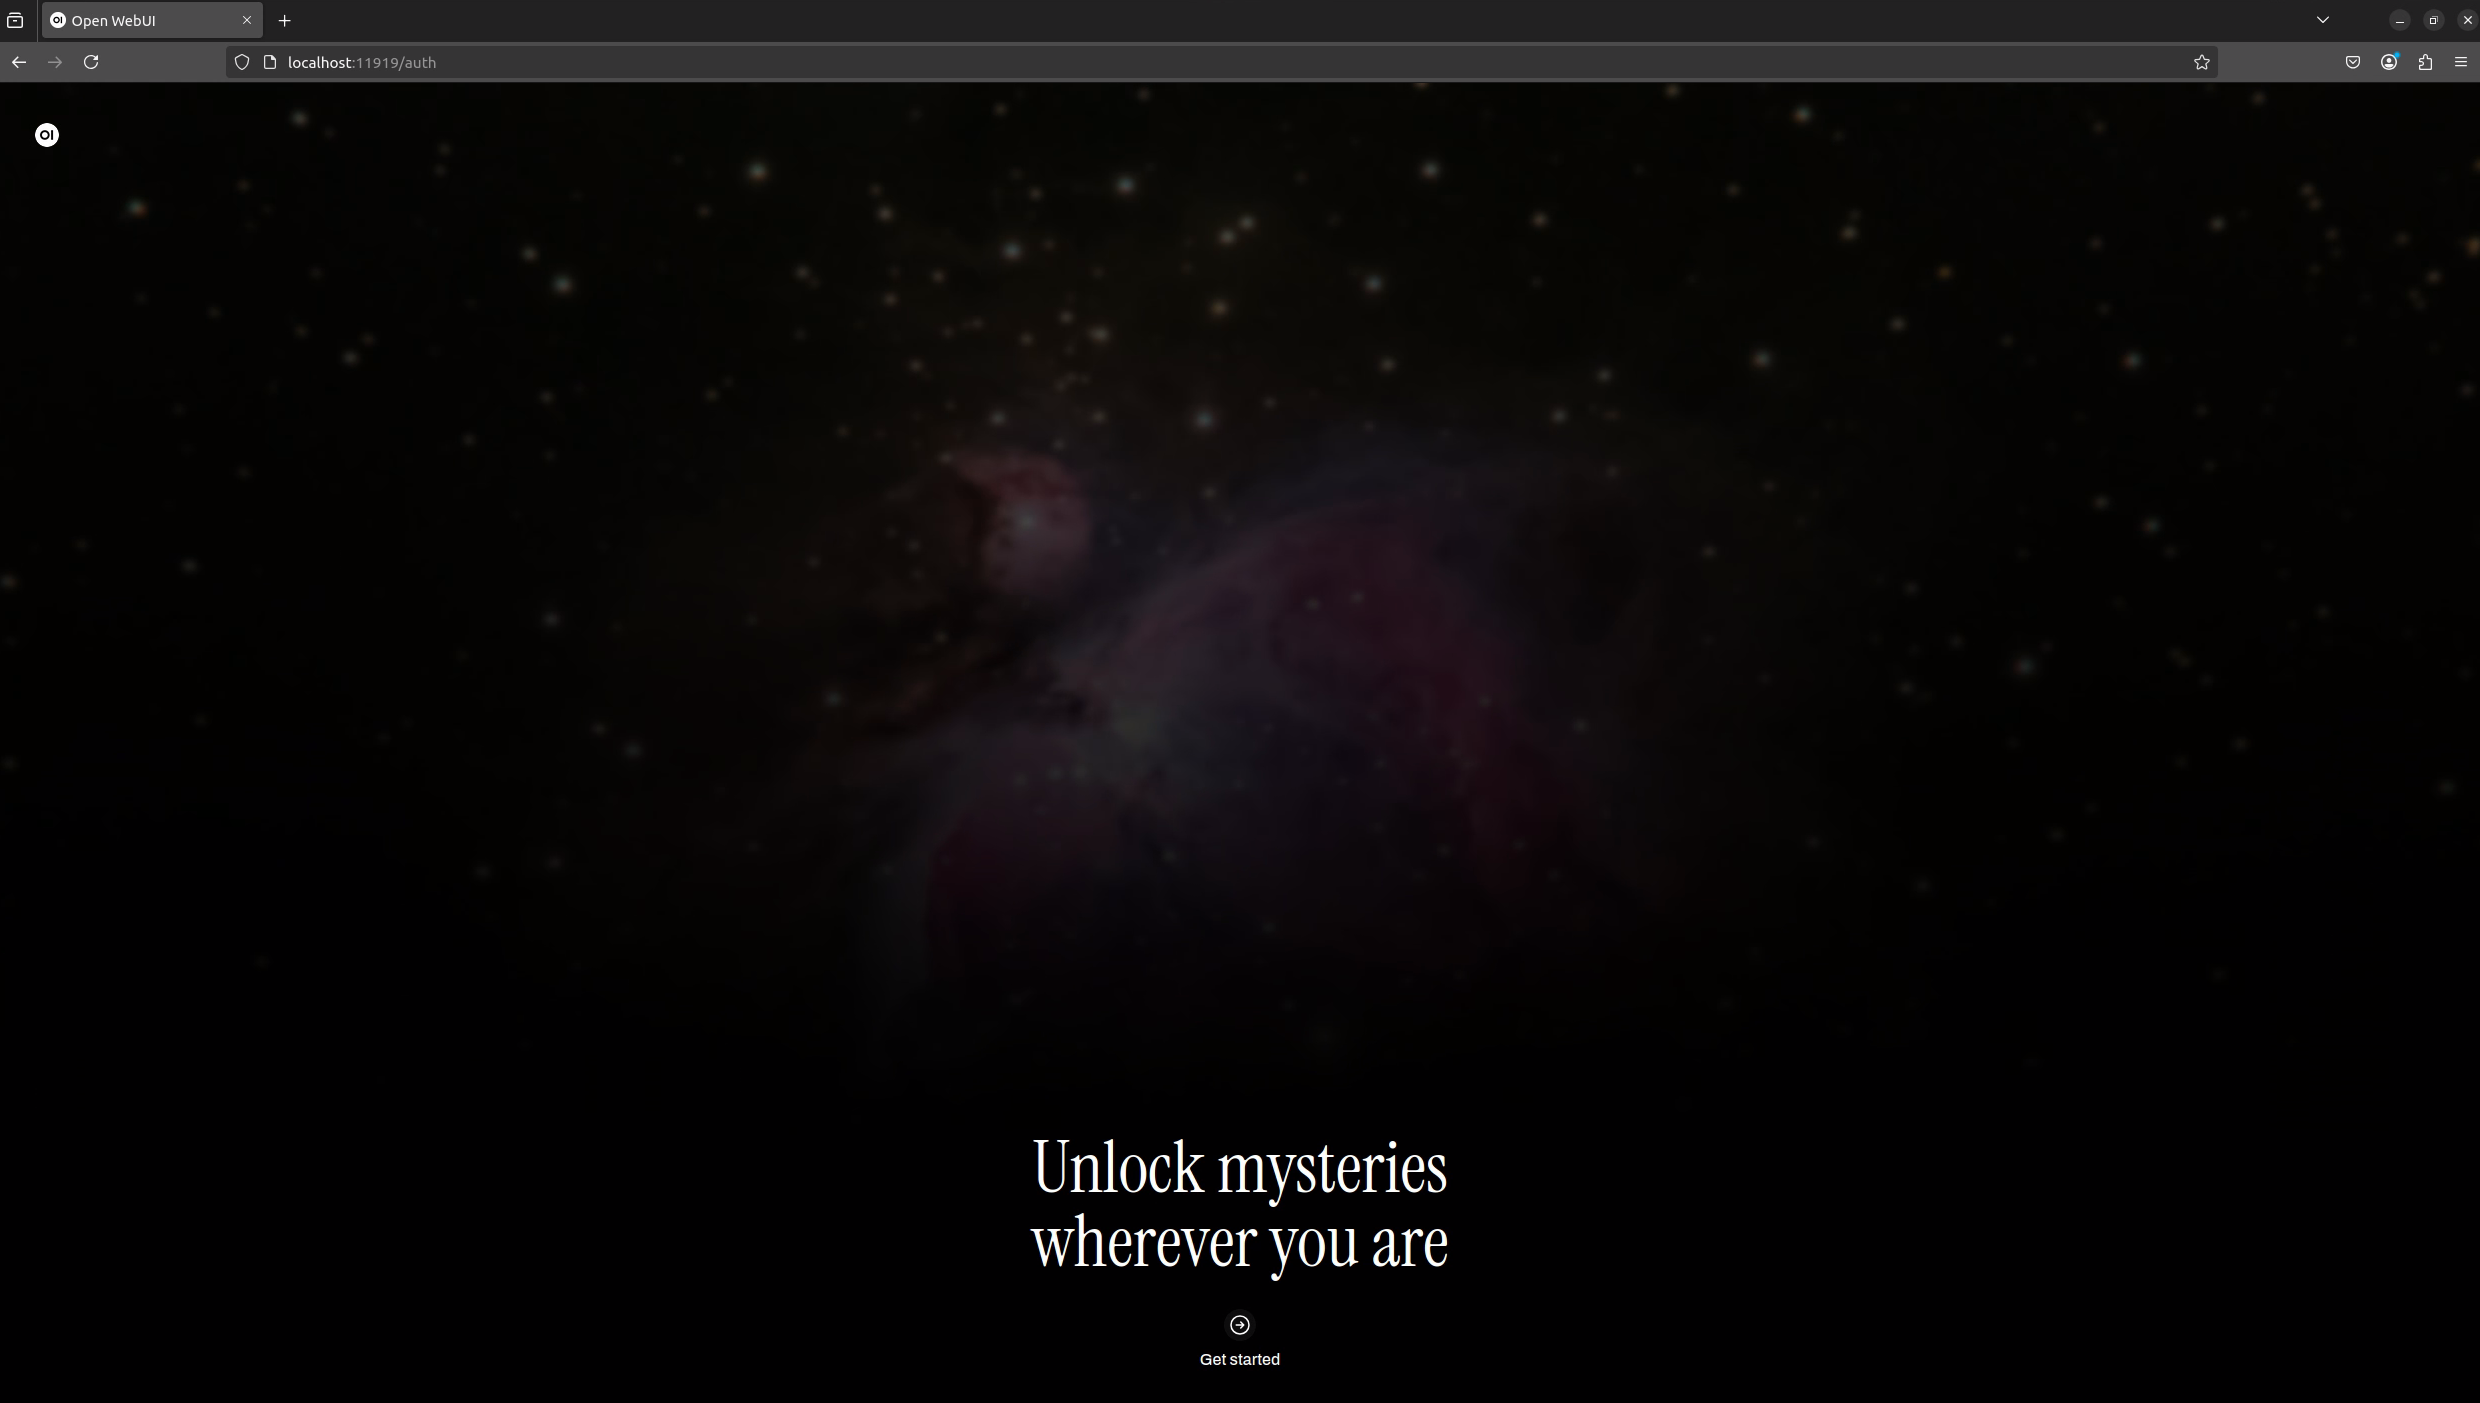
\includegraphics[width=0.8\linewidth]{images/Pasted image 20250304171521.png}
    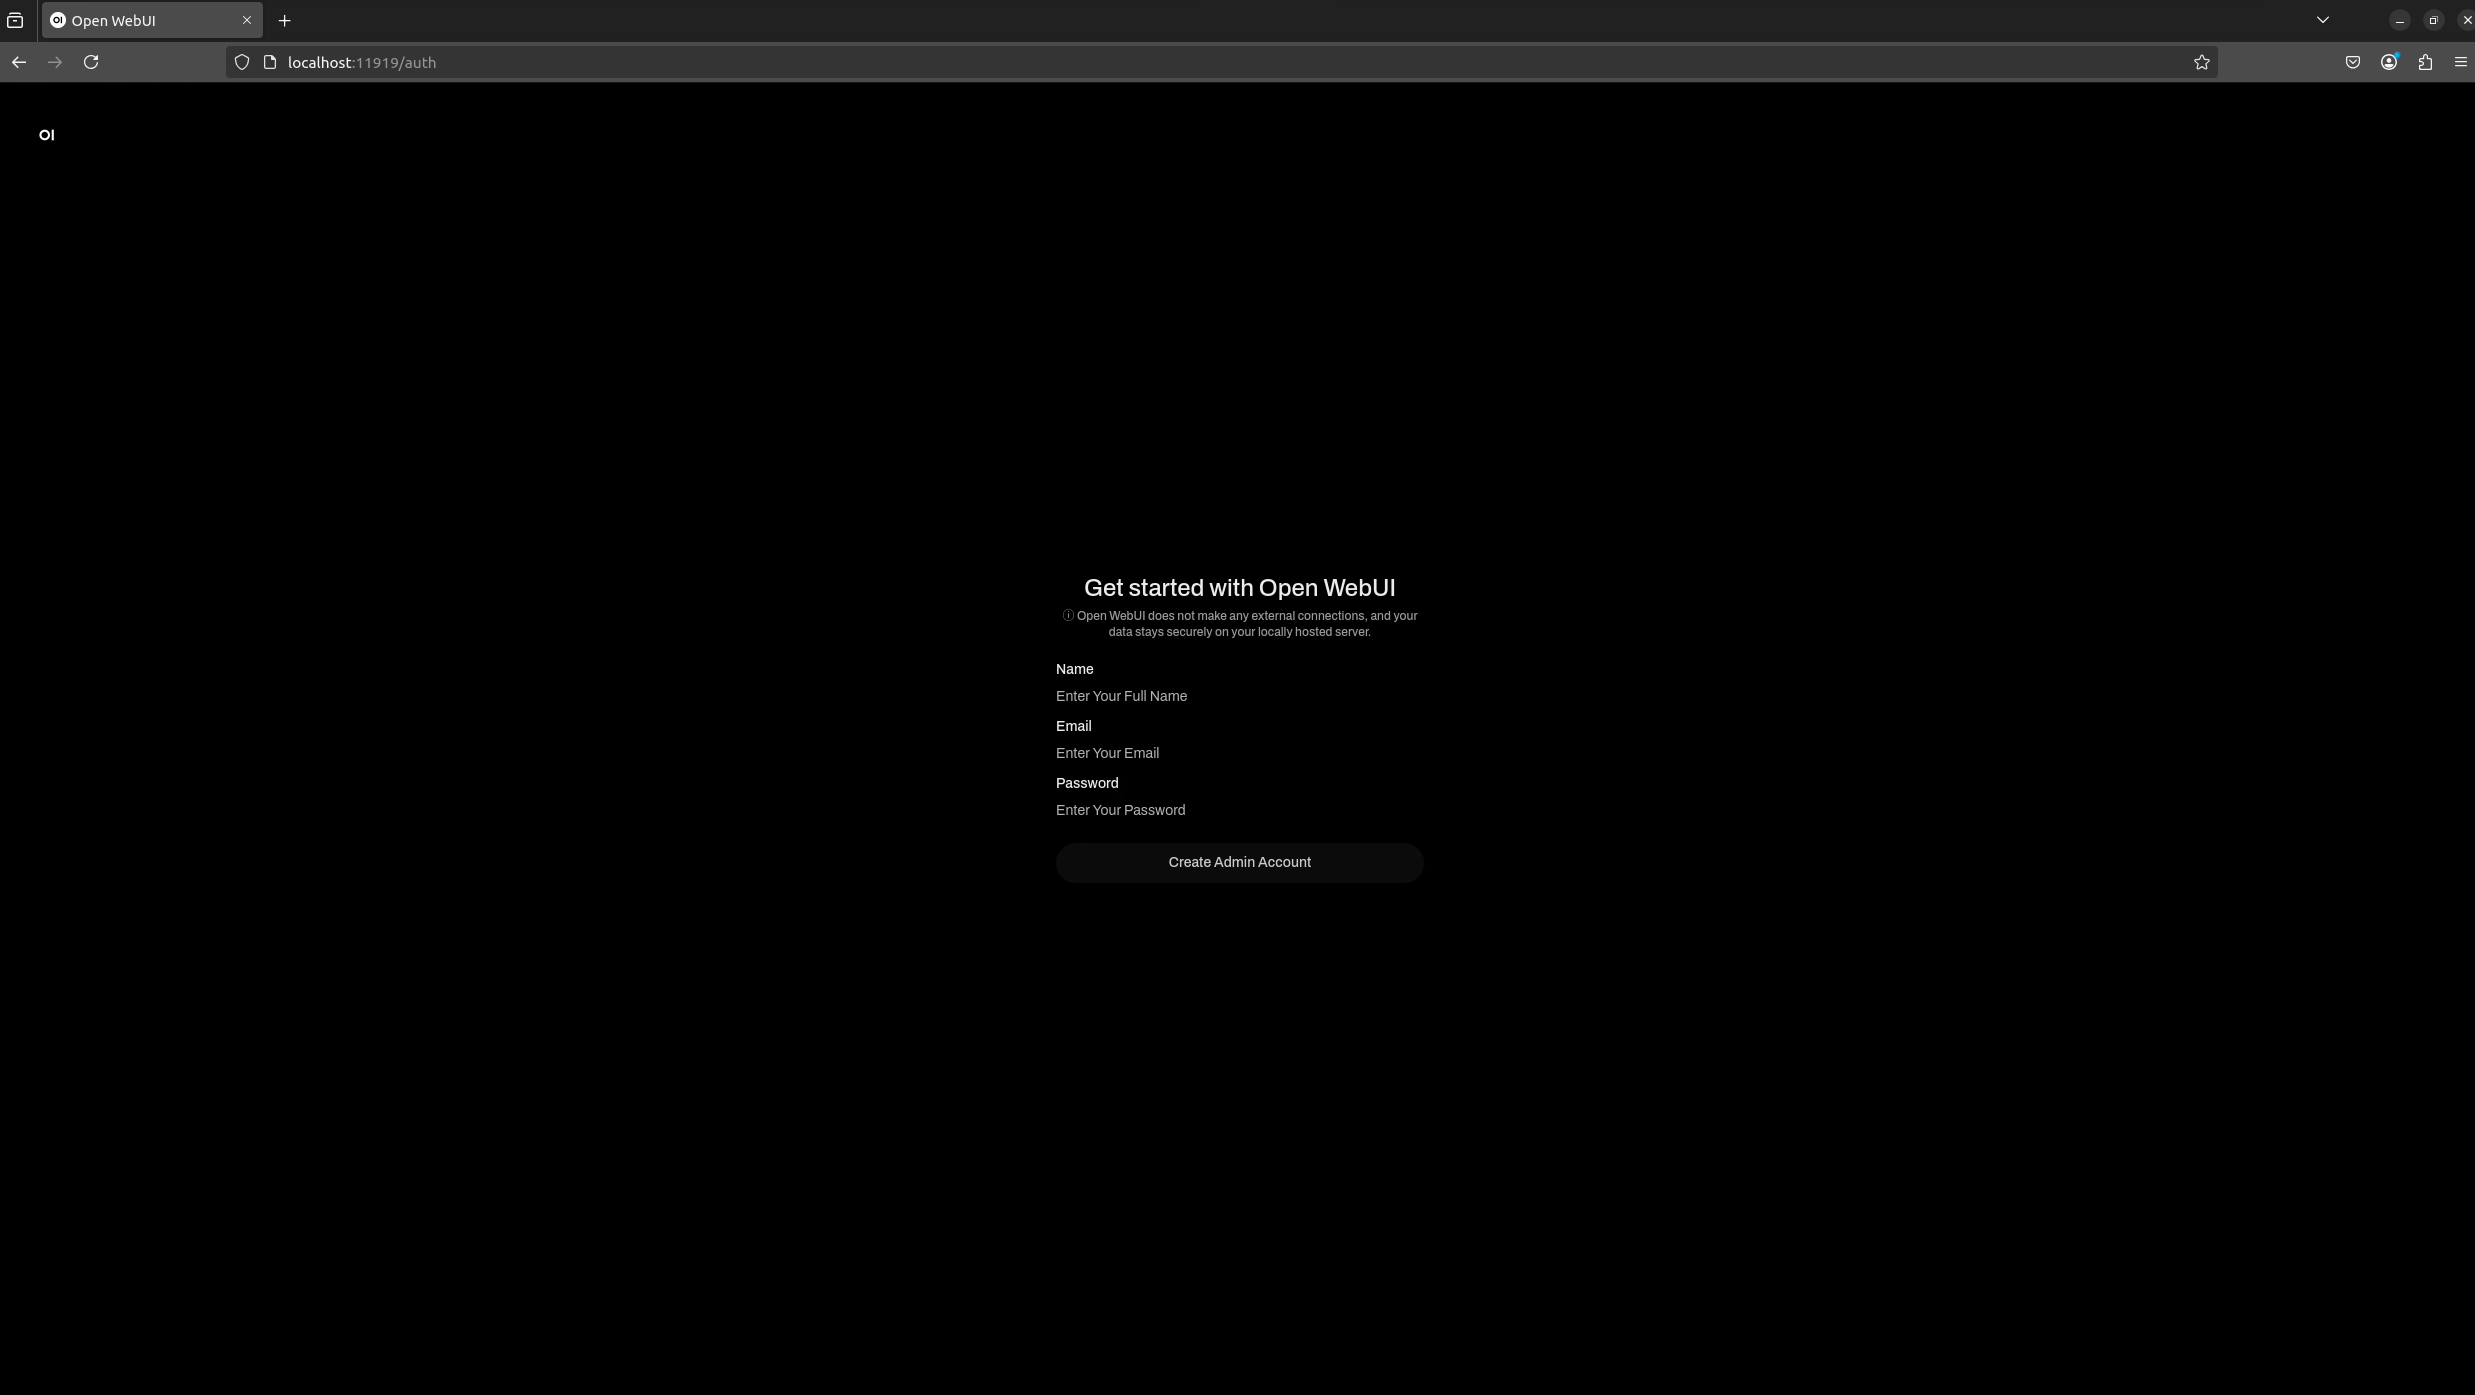
\includegraphics[width=0.8\linewidth]{images/Pasted image 20250304171548.png}
\end{figure}

ログインすると,以下の画面が表示される:
\begin{figure}[H]
    \centering
    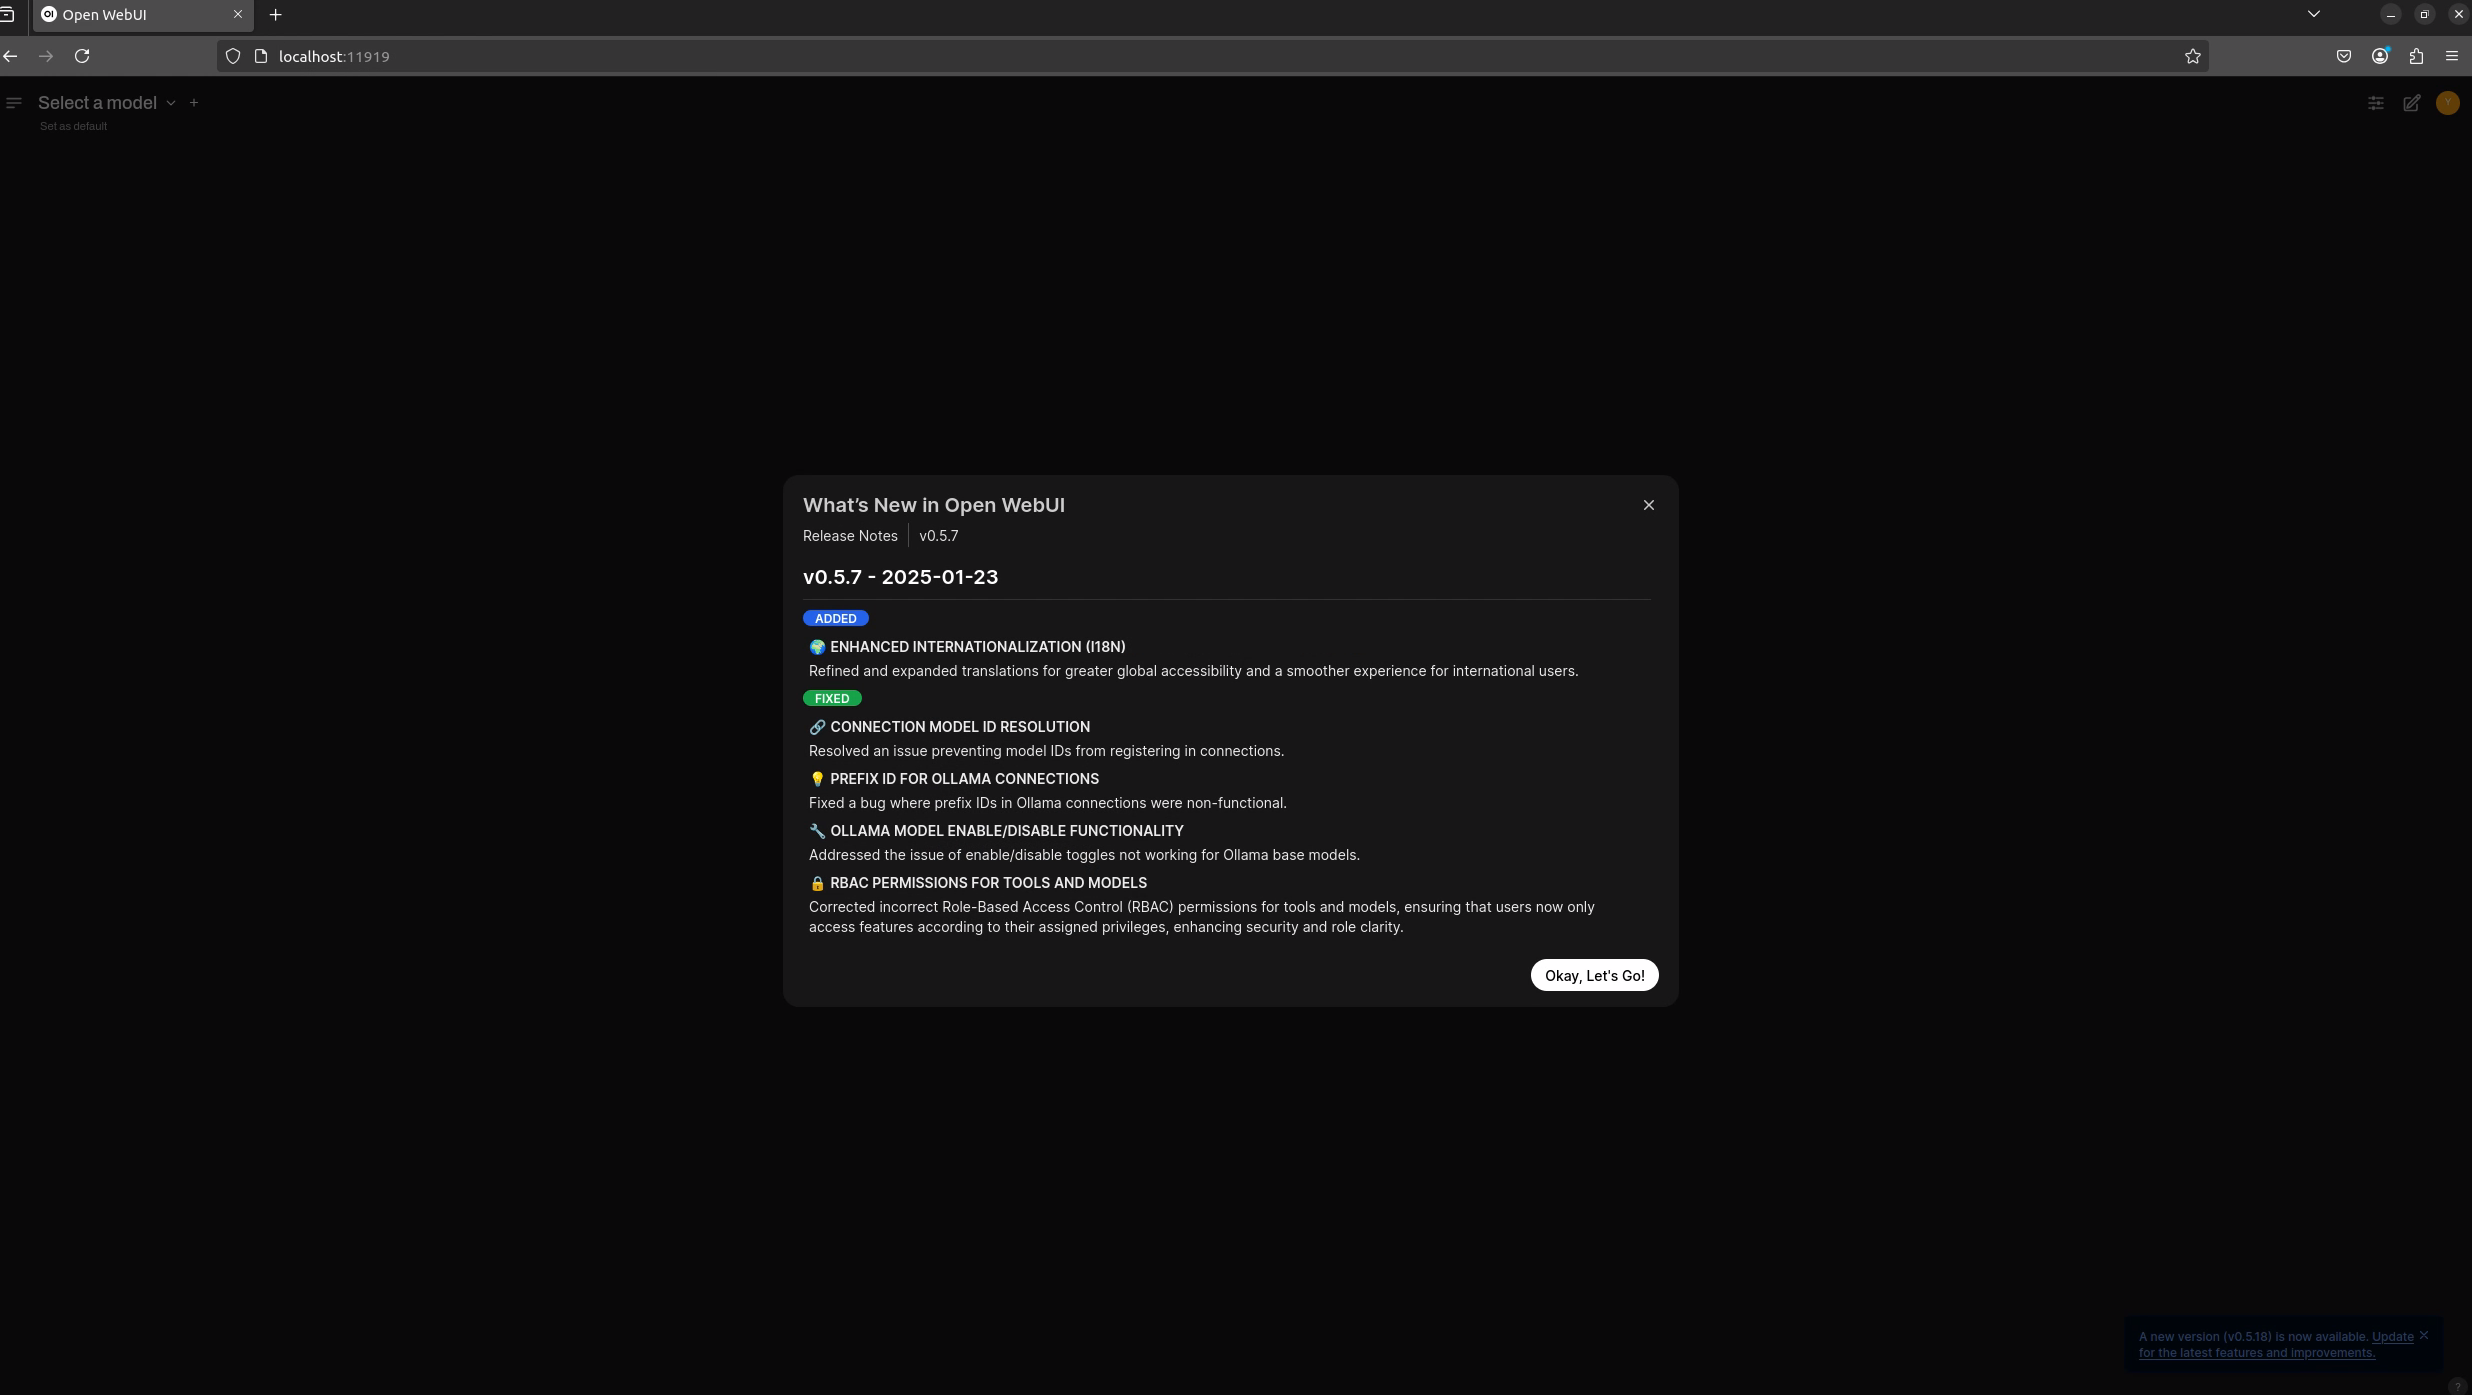
\includegraphics[width=0.8\linewidth]{images/Pasted image 20250304171722.png}
\end{figure}

この時点では,モデルリストは空である.

\begin{figure}[H]
    \centering
    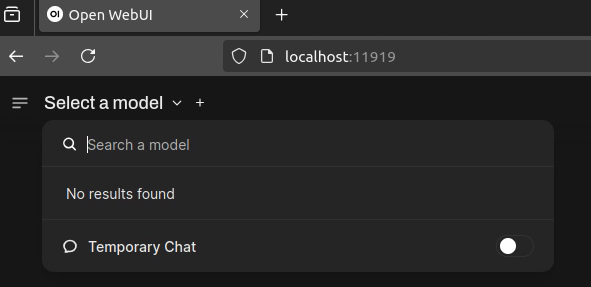
\includegraphics[width=0.8\linewidth]{images/Pasted image 20250304171753.png}
\end{figure}

\paragraph{注意} 長時間GPUを使用しない場合,NVIDIAのドライバがGPUとの接続を自動で切断し,推論速度が大幅に低下する場合がある(CPU推論に切り替わる).その際は,以下のコマンドでコンテナを再起動すること.
\begin{lstlisting}[language=bash]
docker restart open-webui-ollama
\end{lstlisting}

\section{ローカルデプロイしたOpen WebUI(Local Deployment)の使用方法}
LLMとの対話には,まず\href{https://ollama.com/search}{Ollamaサポートモデル一覧}から適切なモデルを選択する.例えば「deepseek-r1」シリーズを使用する場合,ウェブページで異なるパラメータサイズのGPU MEM使用量を確認し,自身の環境に合ったモデルを選択する.もし「deepseek-r1:14b」モデルを使用する場合は以下のコマンドを実行する:

\begin{lstlisting}[language=bash]
docker exec -it open-webui-ollama ollama run deepseek-r1:14b
\end{lstlisting}

\paragraph{コマンドパラメータ解説}
\begin{itemize}
\item \texttt{exec}: コンテナ内でコマンドを実行.コンテナ内で特定のコマンドを実行するためのサブコマンド.
\item \texttt{-it}: インタラクティブモード.リアルタイムのダウンロード進捗表示と対話型インタフェースを有効化.
\item \texttt{open-webui-ollama}: 対象コンテナ名の指定.デプロイ時に設定したコンテナ名と一致させる必要がある.
\item \texttt{ollama run deepseek-r1:14b}: コンテナ環境内で実行するコマンド.モデルのダウンロードと実行を同時に実施.
\end{itemize}

このコマンドにより「deepseek-r1:14b」モデルが自動的にダウンロードされる.コマンドラインでの対話例:
\begin{lstlisting}[language=bash]
% docker exec -it open-webui-ollama ollama run deepseek-r1:14b
>>> How do you do?
<think>

</think>

Hi! I'm DeepSeek-R1, an artificial intelligence assistant created by
DeepSeek. For comprehensive details about our models and products, we
invite you to consult our official documentation.

>>> /bye
\end{lstlisting}

いま\texttt{http://localhost:11919} にアクセスすると,下のような画面が表示される.

\begin{figure}[H]
    \centering
    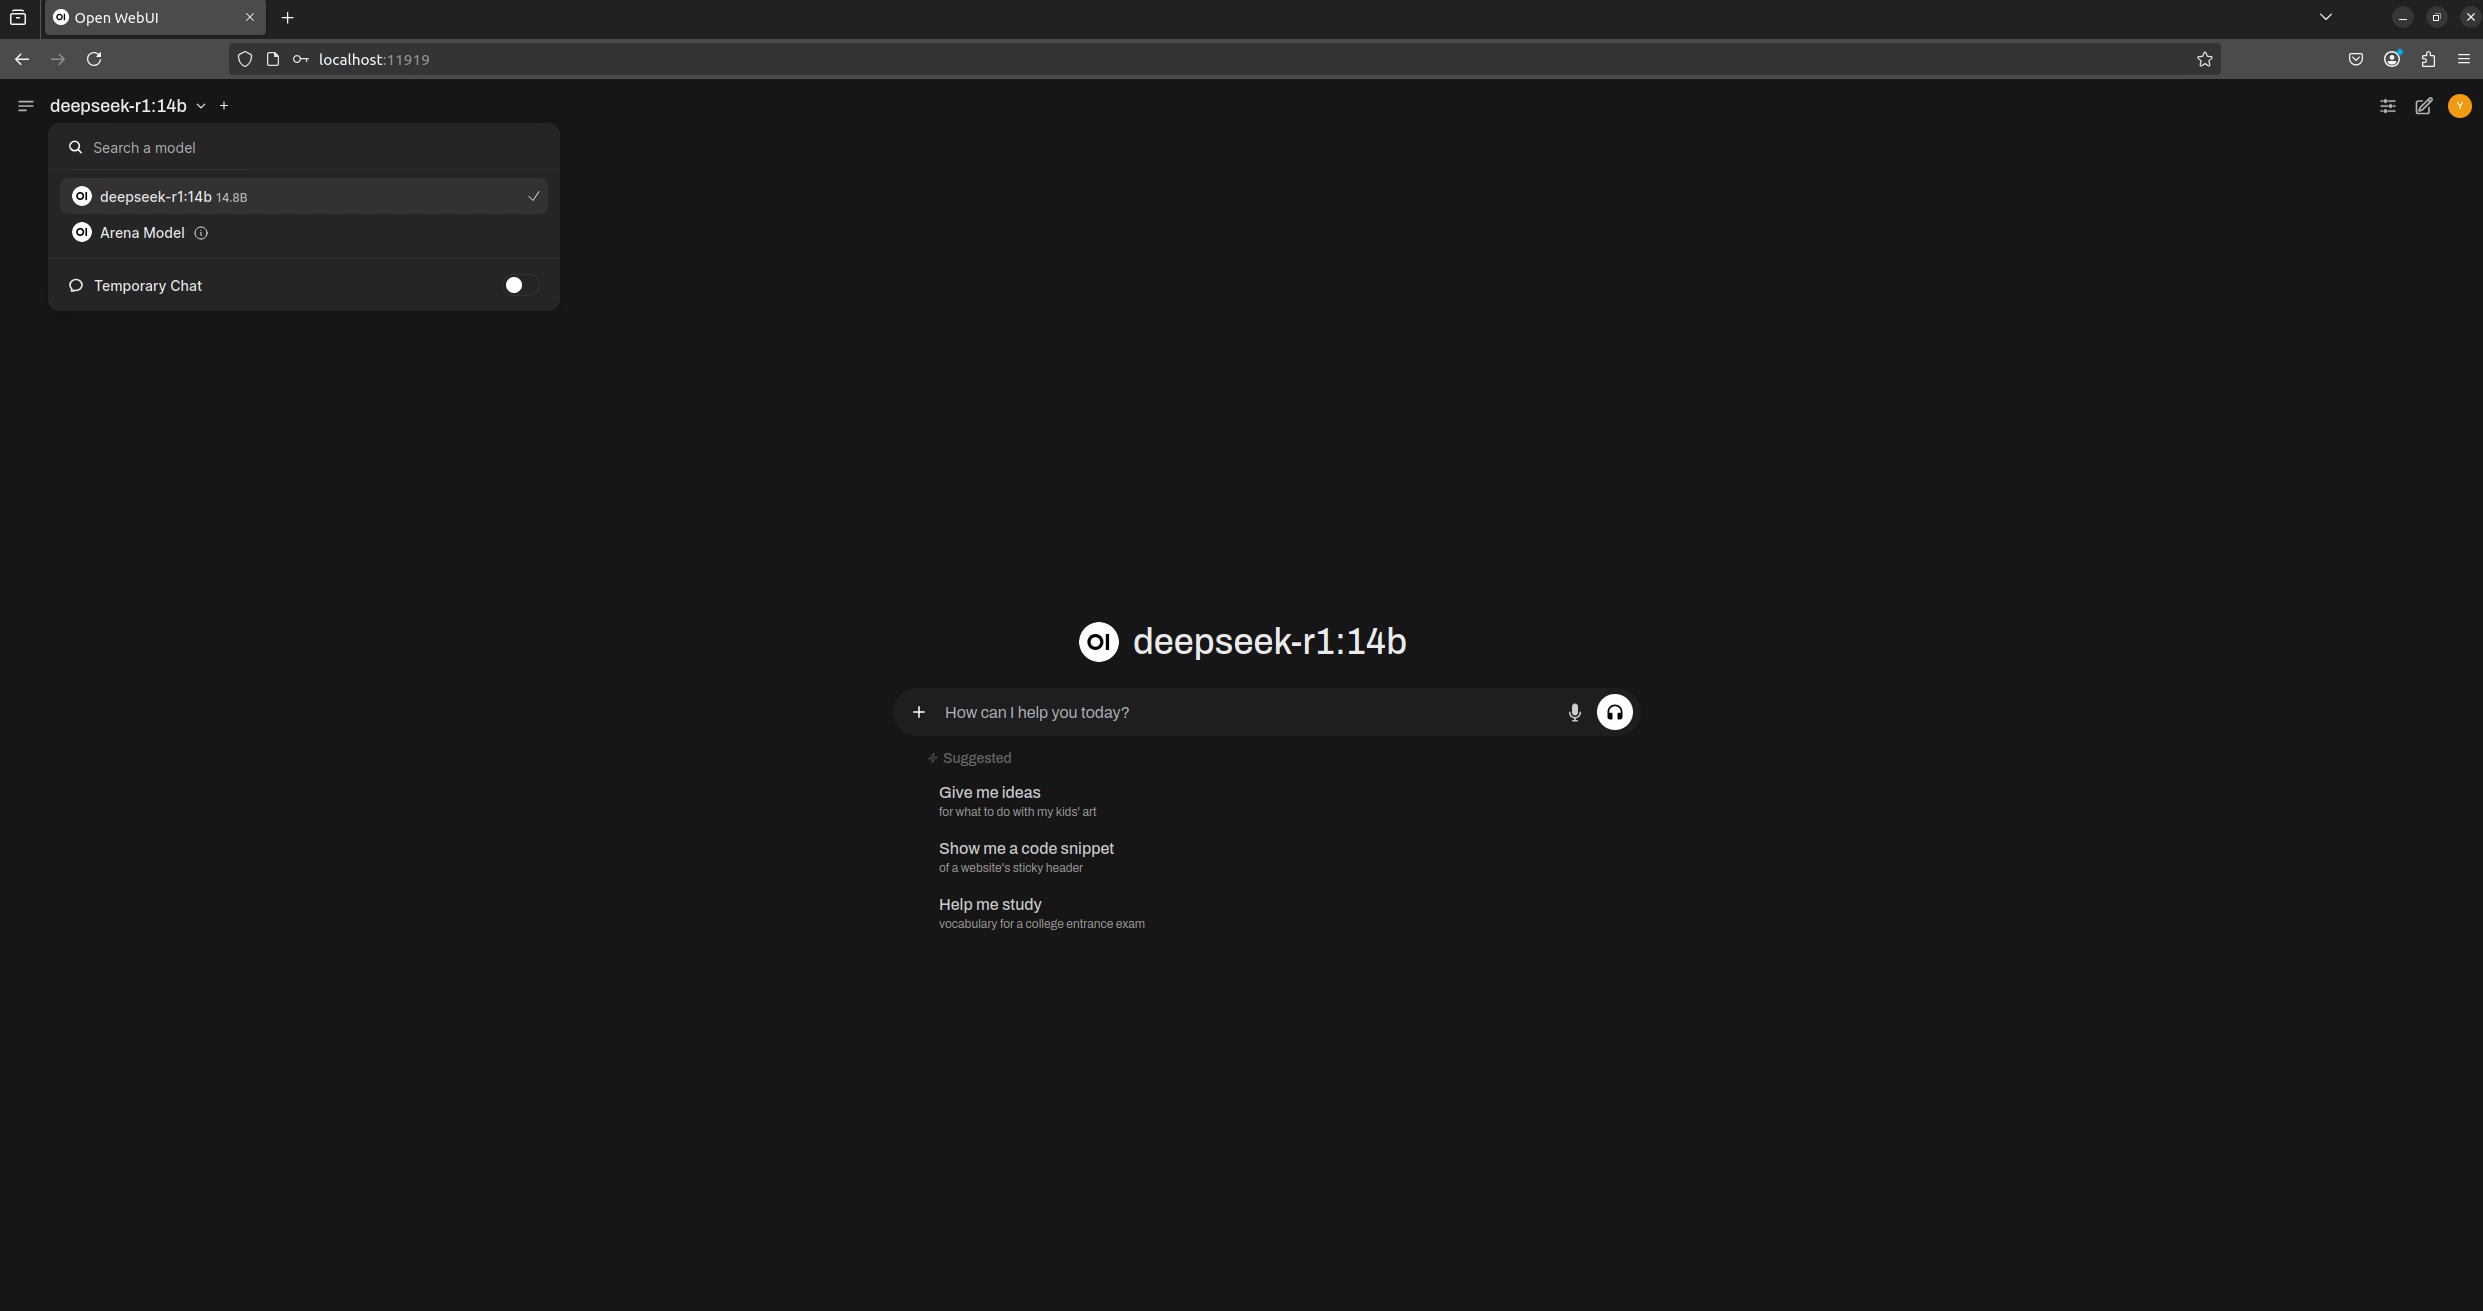
\includegraphics[width=0.8\linewidth]{images/Pasted image 20250304170628.png}
\end{figure}

\paragraph{高度な設定}
右上のモデルパラメータ設定では以下の調整ができる:
\begin{itemize}
\item 温度(Temperature): 生成テキストのランダム性を制御.
\item 最大トークン数(Max Tokens): 生成テキストの長さを制限.
\item トップP(Top-P): 確率分布に基づくサンプリング範囲を調整.
\end{itemize}

その他の機能(ユーザ権限管理,ネットワーク検索サービス連携等)は設定メニューで確認できる.詳細な機能探索はユーザ自身で活用してください.

\paragraph{技術的注意点}
\begin{itemize}
\item 「docker exec」コマンド実行前に対象コンテナ(open-webui-ollama)が正常に起動していることが必要.
\item 「ollama run」コマンドはモデル未ダウンロード時に自動取得するが,1-30分程度要する場合がある(ネットワーク速度に依存).
\item モデルダウンロードにはGPU MEMとディスク容量が十分にあることを確認すること.メモリ不足時はより小さいモデル(例:7B)の選択を推奨.
\end{itemize}

\section{\texttt{docker-compose}を使用したアプリケーションのデプロイ(Overleafを例として)}

\texttt{docker-compose}は、Docker公式が提供するツールであり、複数のコンテナを用いたDockerアプリケーションを定義・管理するために使用される。YAMLファイルを使用して、アプリケーションに必要なすべてのサービスを設定し、単一のコマンドでサービスの起動や停止が可能である。この機能は、Webサービス、データベース、キャッシュなど、複数の相互依存するサービスを持つアプリケーションに特に有用である。

Overleafは、リアルタイムの共同編集とコンパイル機能を提供するオンラインLaTeXエディタである。その\textbf{Community Edition(コミュニティ版)}はオープンソースとして公開されており、自己ホスティングが可能である。公式のオンライン版では多人数でのコラボレーション機能を利用するには課金が必要だが、コミュニティ版をローカルサーバーにデプロイすれば、この制約なしに利用できる。

\subsection{\texttt{docker-compose}を用いたOverleafのデプロイ}
\texttt{docker-compose}は関連する設定情報をディレクトリ単位で管理します。本チュートリアルで使用する設定ファイルは以下のリポジトリから取得可能です:

\begin{lstlisting}[language=bash]
git clone https://github.com/watashihame/25OnCampusJob.git
\end{lstlisting}

\paragraph{リポジトリを使用しない方法}
\begin{enumerate}
\item 作業ディレクトリの作成
\begin{lstlisting}[language=bash]
mkdir overleaf-test
cd overleaf-test
\end{lstlisting}

\item Overleaf設定ファイルの取得
\begin{lstlisting}[language=bash]
wget https://raw.githubusercontent.com/watashihame/25OnCampusJob/refs/heads/main/overleaf-test/docker-compose.yml
\end{lstlisting}
\end{enumerate}

\paragraph{設定ファイルの解説}
Overleafの設定は\texttt{./overleaf-test}の\texttt{docker-compose.yml}ファイルによって記述されます。
このファイルは3つのコンテナ(\texttt{sharelatex}、\texttt{mongo}、\texttt{redis})を定義しており、起動順序は\texttt{depends\_on}(依存関係)で制御されています。

主要なカスタマイズ項目:
\begin{itemize}
\item ポートマッピング:\texttt{sharelatex}サービスの\texttt{ports}設定(例:\texttt{"80:80"}→\texttt{"8880:80"})
\item 環境変数:各サービスごとの設定パラメータ
\item データ保存先(ボリューム):
  \begin{itemize}
  \item \texttt{./sharelatex\_data}: プロジェクトファイルとコンパイル結果(Project files and build artifacts)
  \item \texttt{./mongo\_data}: MongoDBデータベース(Database storage)
  \item \texttt{./redis\_data}: Redisキャッシュ(In-memory data store)
  \end{itemize}
\end{itemize}

\paragraph{注意}
\begin{itemize}
\item データ保存先の変更は\texttt{volumes}設定を編集
\item 本設定ファイルは簡略化版であり、HTTPS対応やNginxリバースプロキシなどの高度な設定が必要な場合は、\href{https://github.com/overleaf/overleaf/tree/main}{公式リポジトリ}を参照
\item Overleafは現在docker-composeを使用したセルフホスティングを推奨していません(あくまでデモンストレーション目的での使用)
\end{itemize}

設定が完了したら、以下のコマンドでOverleafを起動する:

\begin{lstlisting}[language=bash]
docker compose up -d
\end{lstlisting}

正常に起動すると、以下のようなメッセージが表示される:

\begin{lstlisting}[language=bash]
$ docker compose up -d
[+] Running 3/3
  Container mongo-test       Healthy   10.7s
  Container redis-test       Started    0.2s
  Container sharelatex-test  Started   10.9s
\end{lstlisting}

停止する場合は以下のコマンドを使用する:

\begin{lstlisting}[language=bash]
docker compose down
\end{lstlisting}

また、再起動する場合は以下のコマンドを使用する:

\begin{lstlisting}[language=bash]
docker compose restart
\end{lstlisting}

\subsection{Overleafサービスの初期設定}

起動後、\texttt{http://localhost:8808} にアクセスすると、Overleafの管理画面に入ることができる。

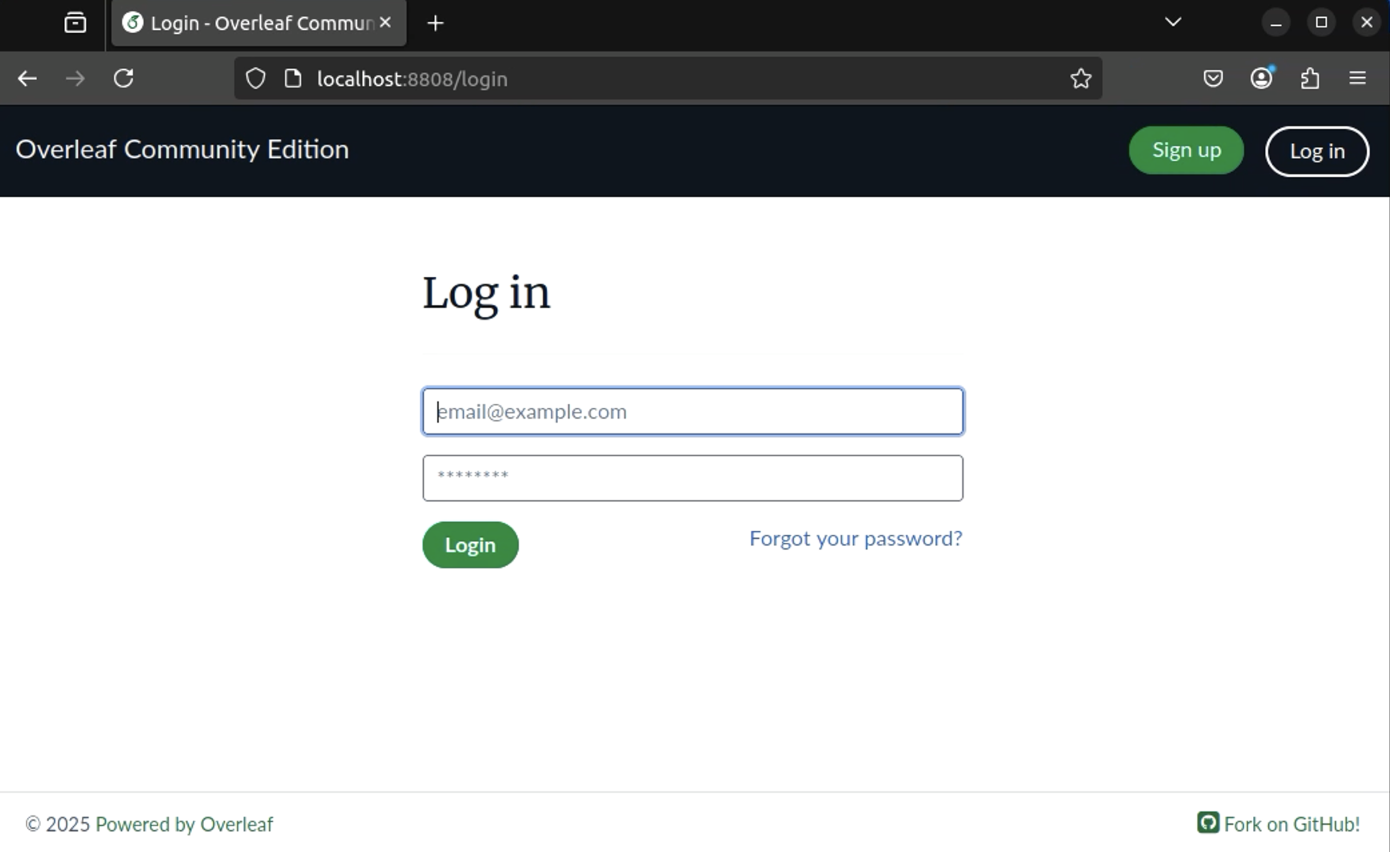
\includegraphics[width=0.8\linewidth]{images/Pasted image 20250307155416.png}

管理者アカウントを作成するため、\\ \texttt{http://localhost:8808/launchpad} にアクセスする。

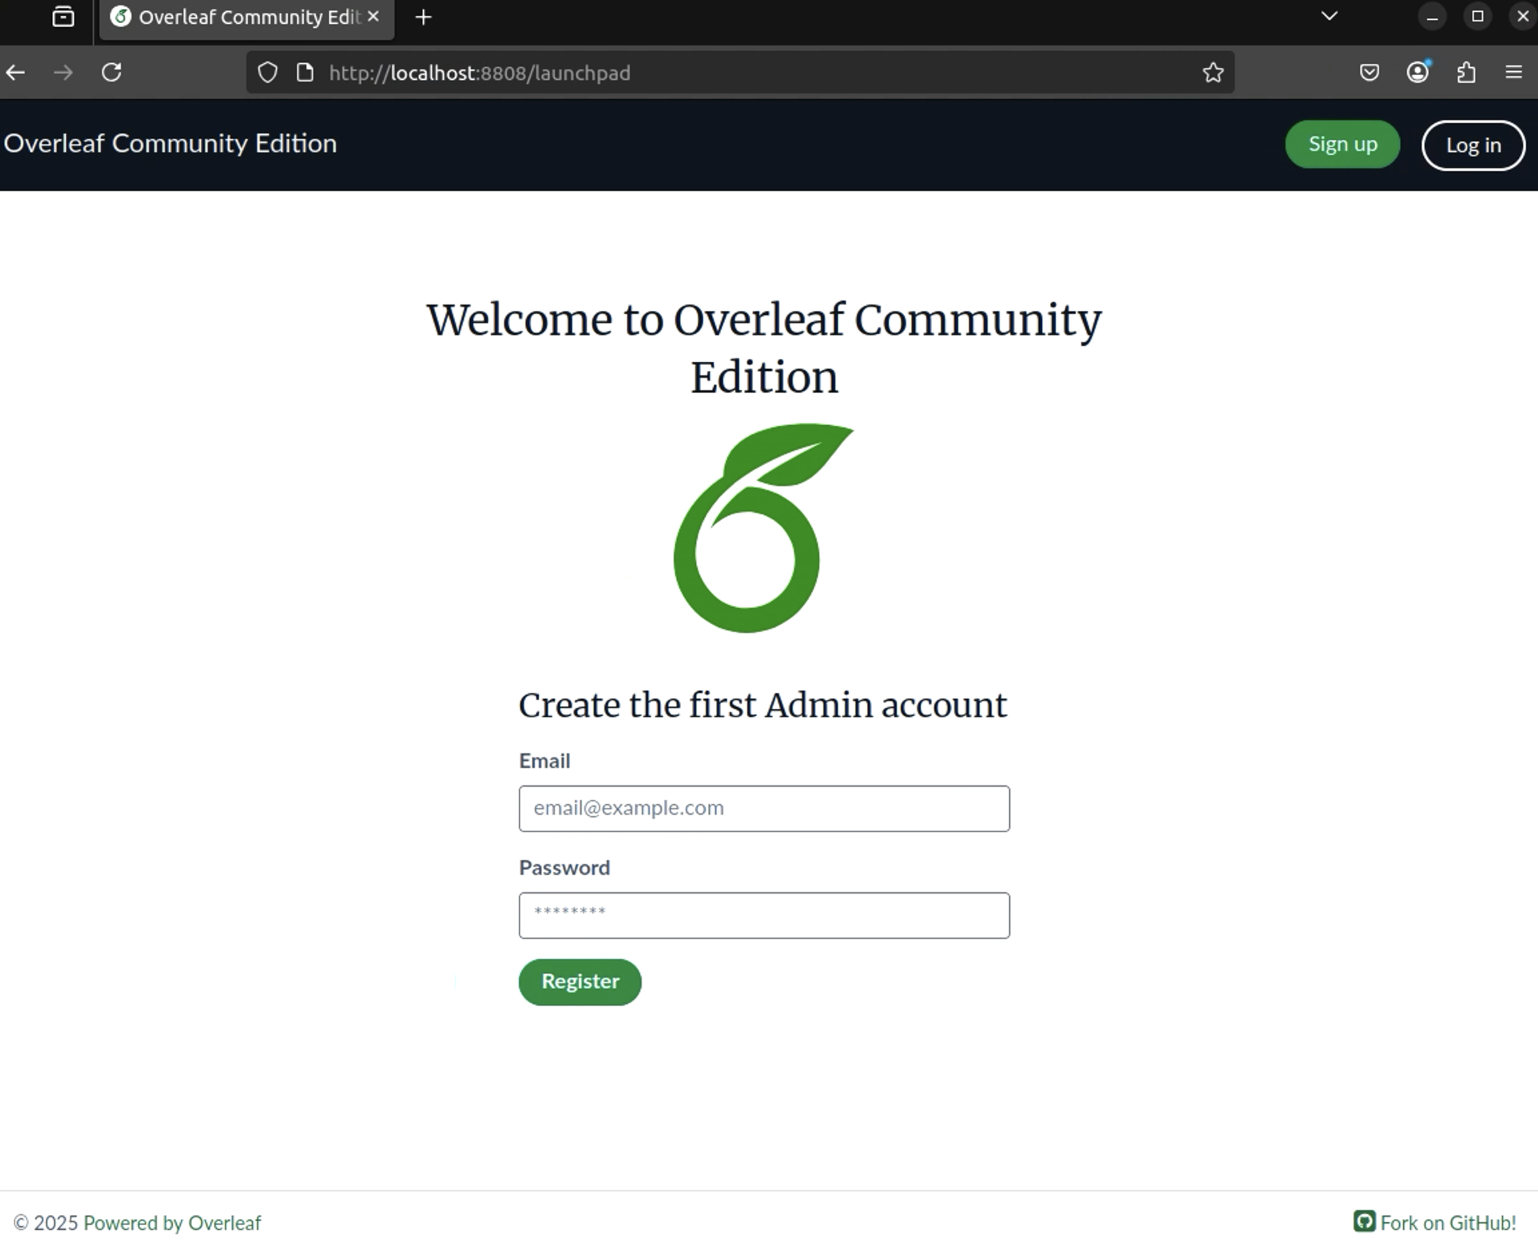
\includegraphics[width=0.8\linewidth]{images/Pasted image 20250307160444.png}

登録後、ログイン画面に遷移し、作成したアカウントでログインできる。

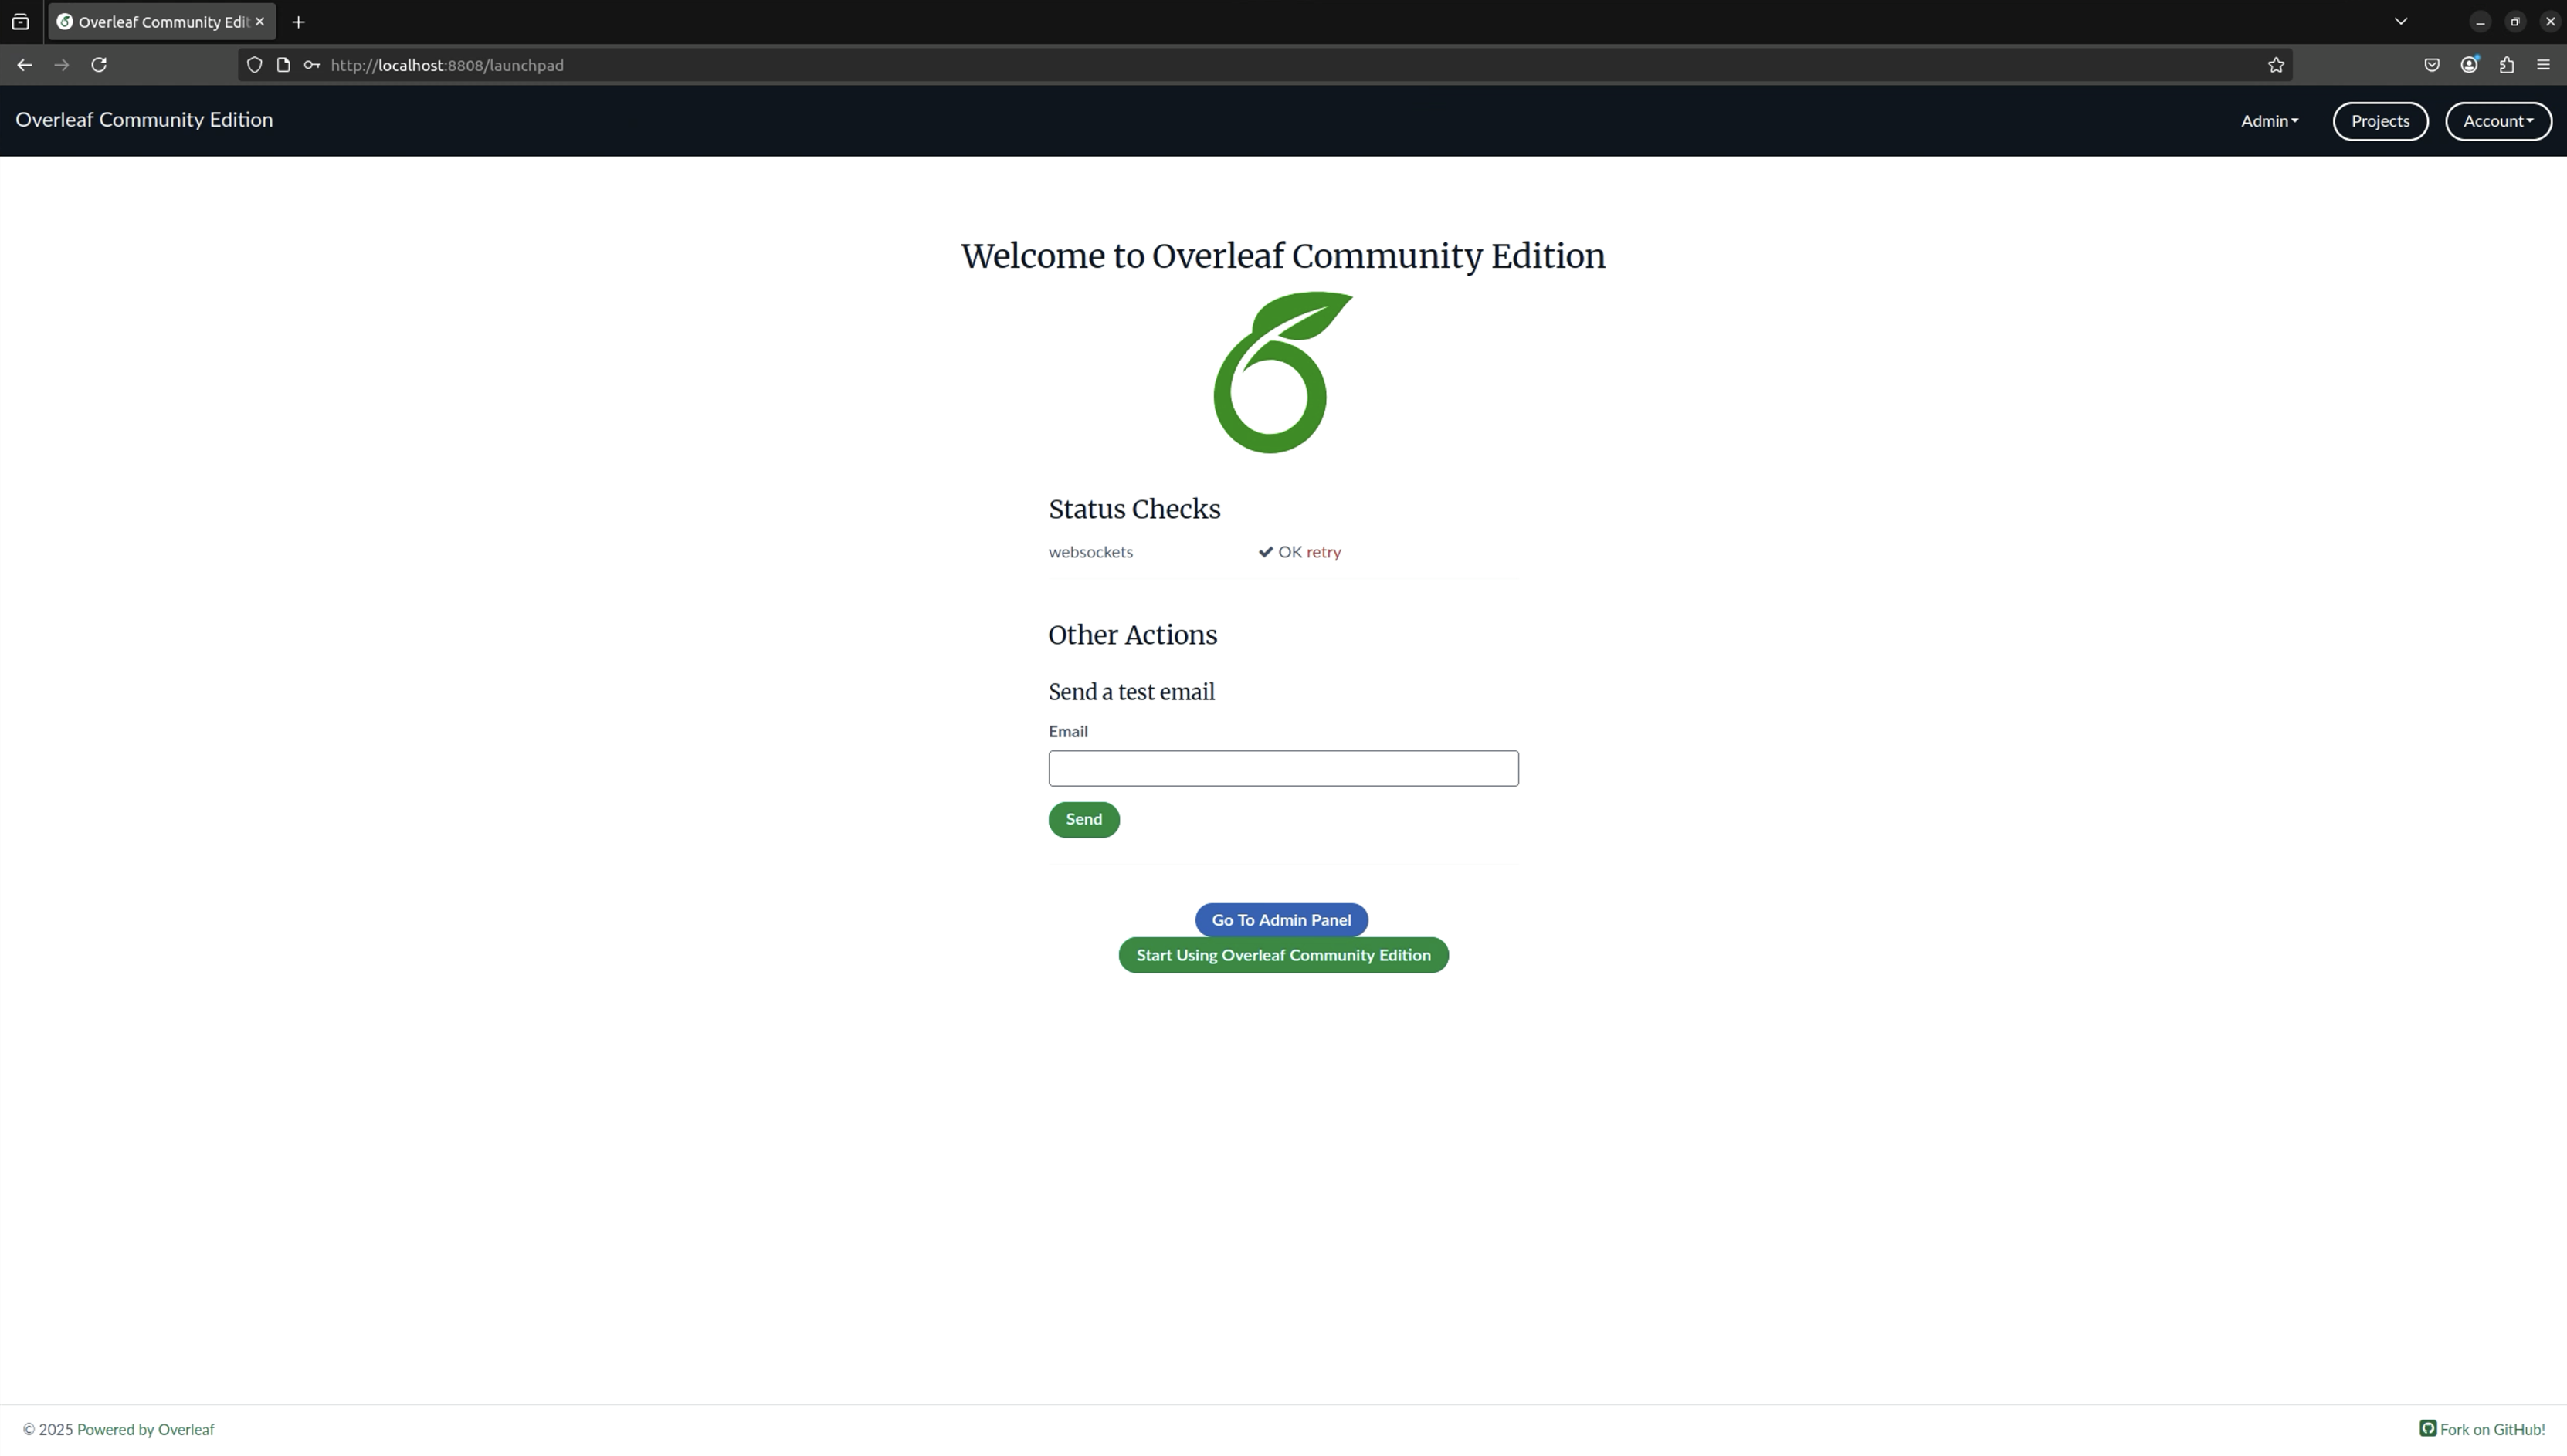
\includegraphics[width=0.8\linewidth]{images/Pasted image 20250307160656.png}

その後、英語の簡単な文書を作成できる。

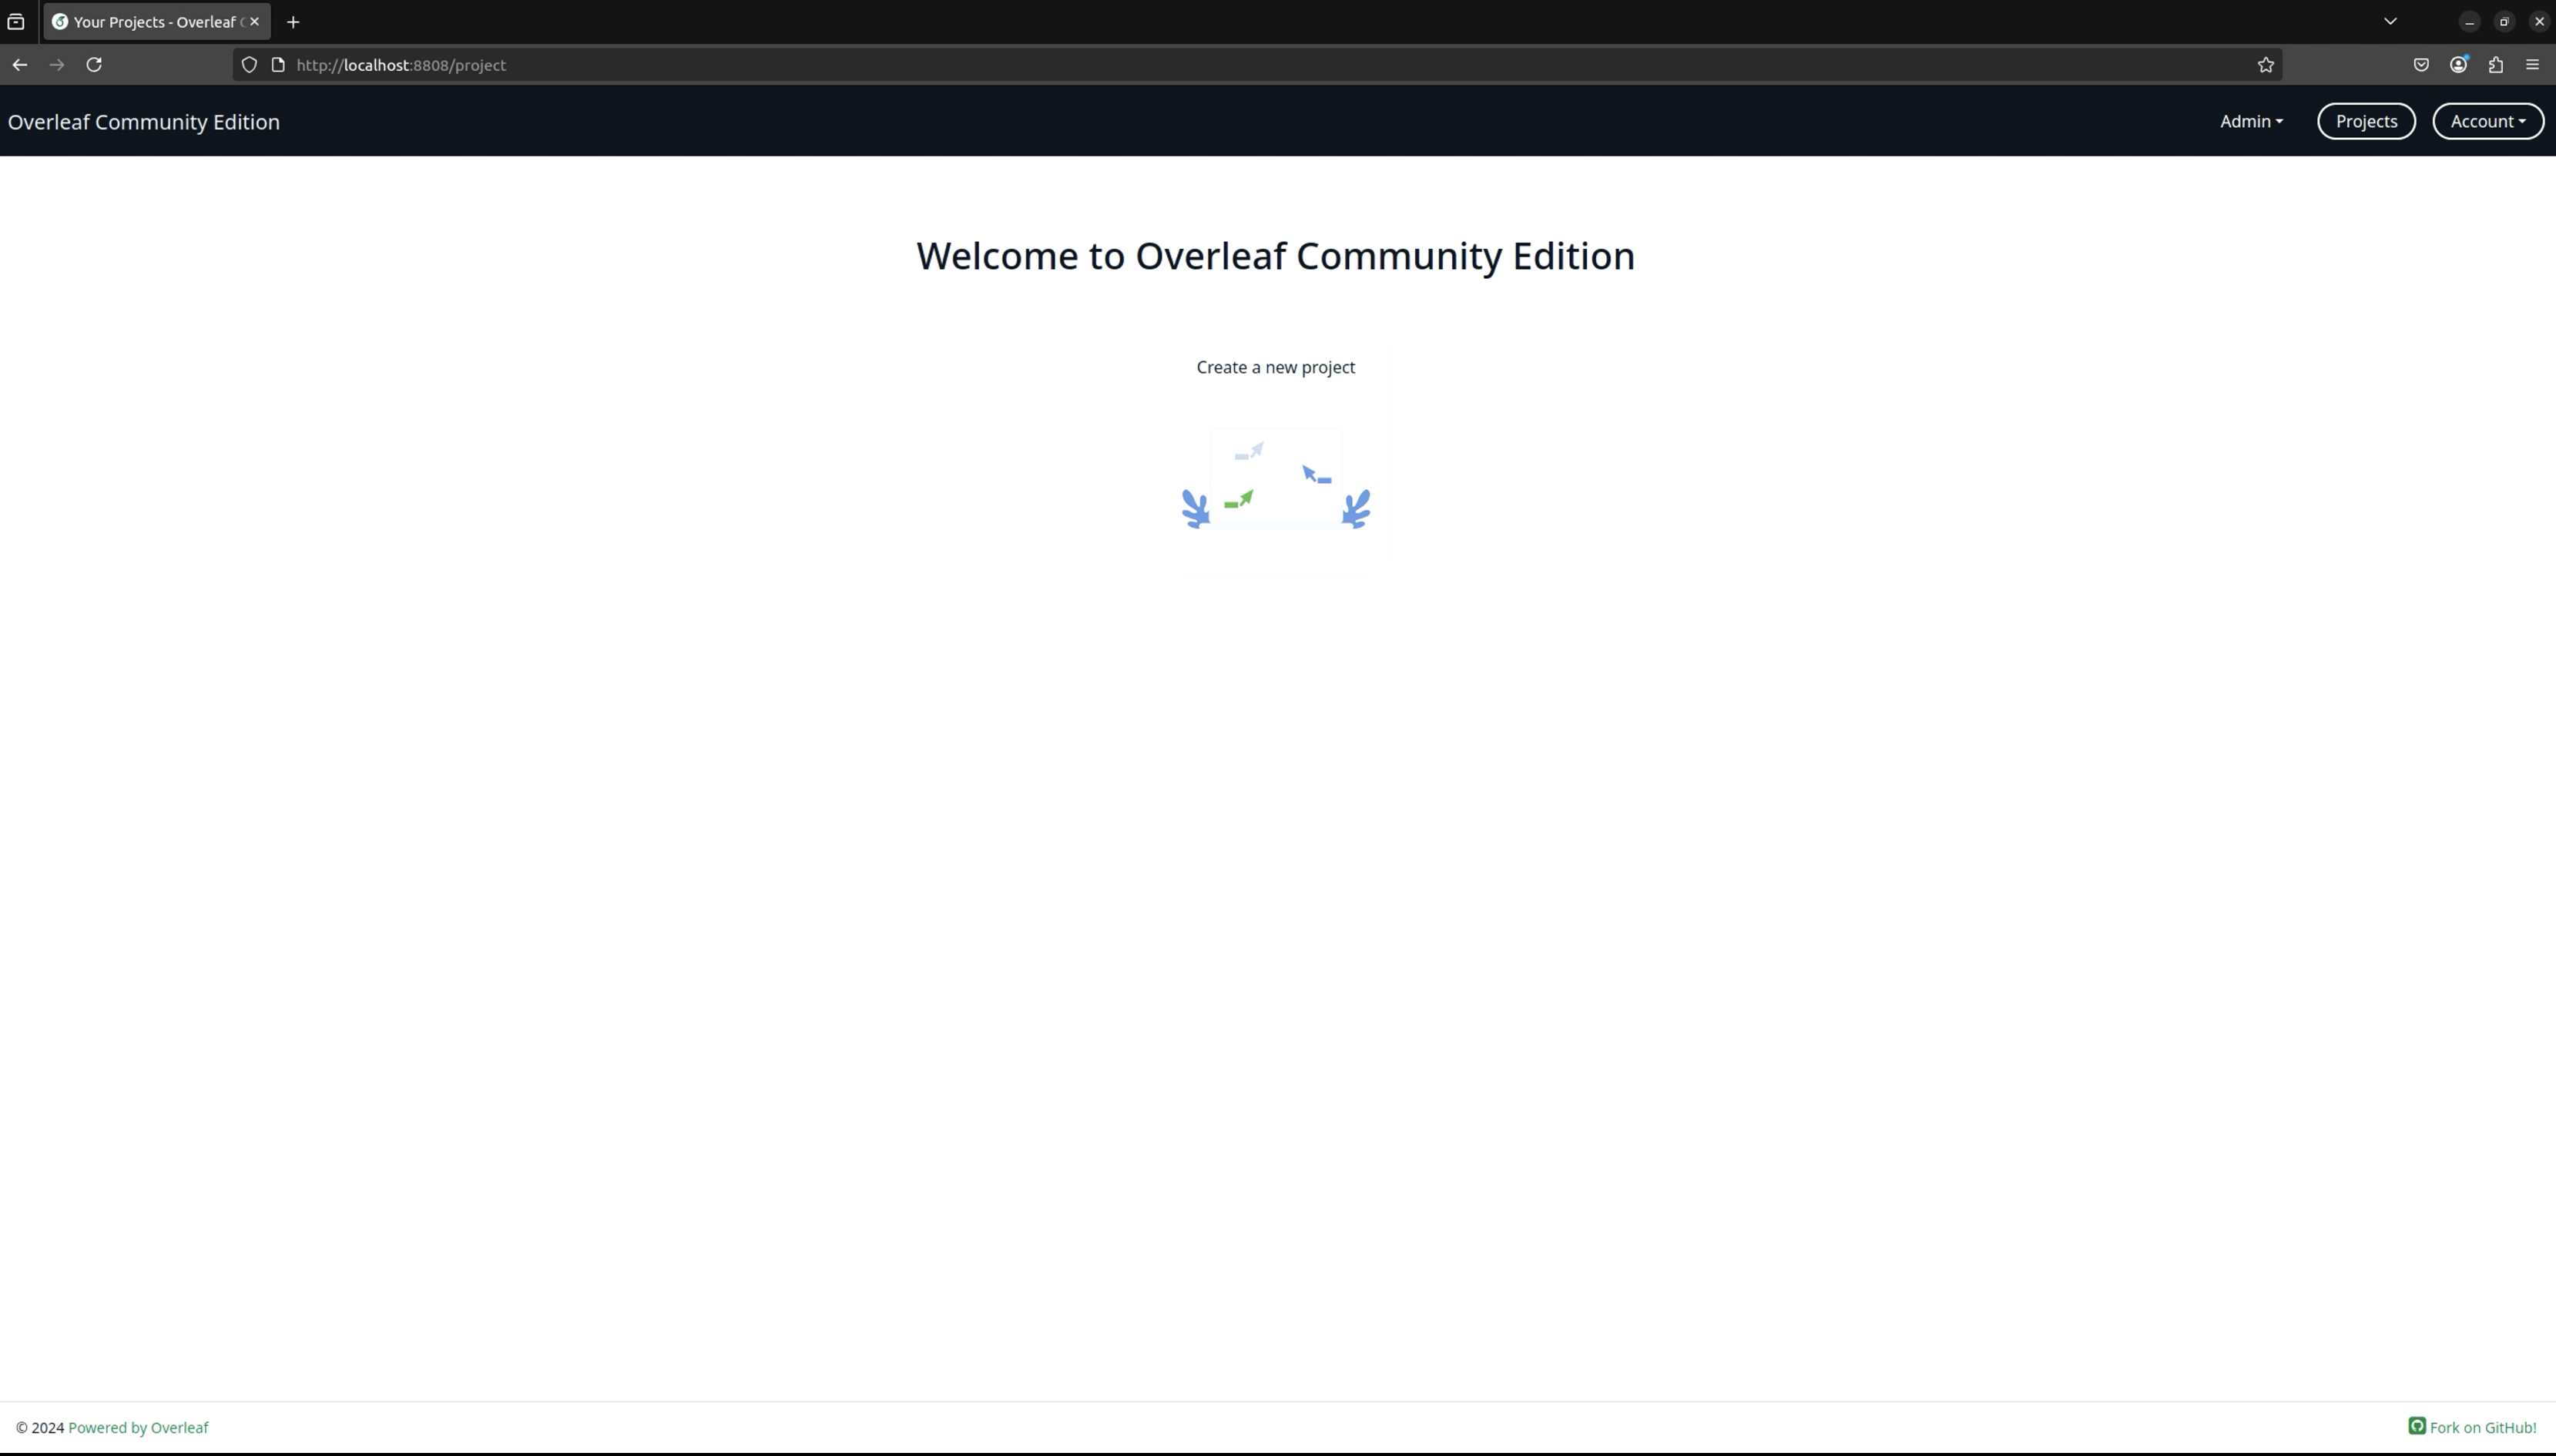
\includegraphics[width=0.8\linewidth]{images/Pasted image 20250307160922.png}

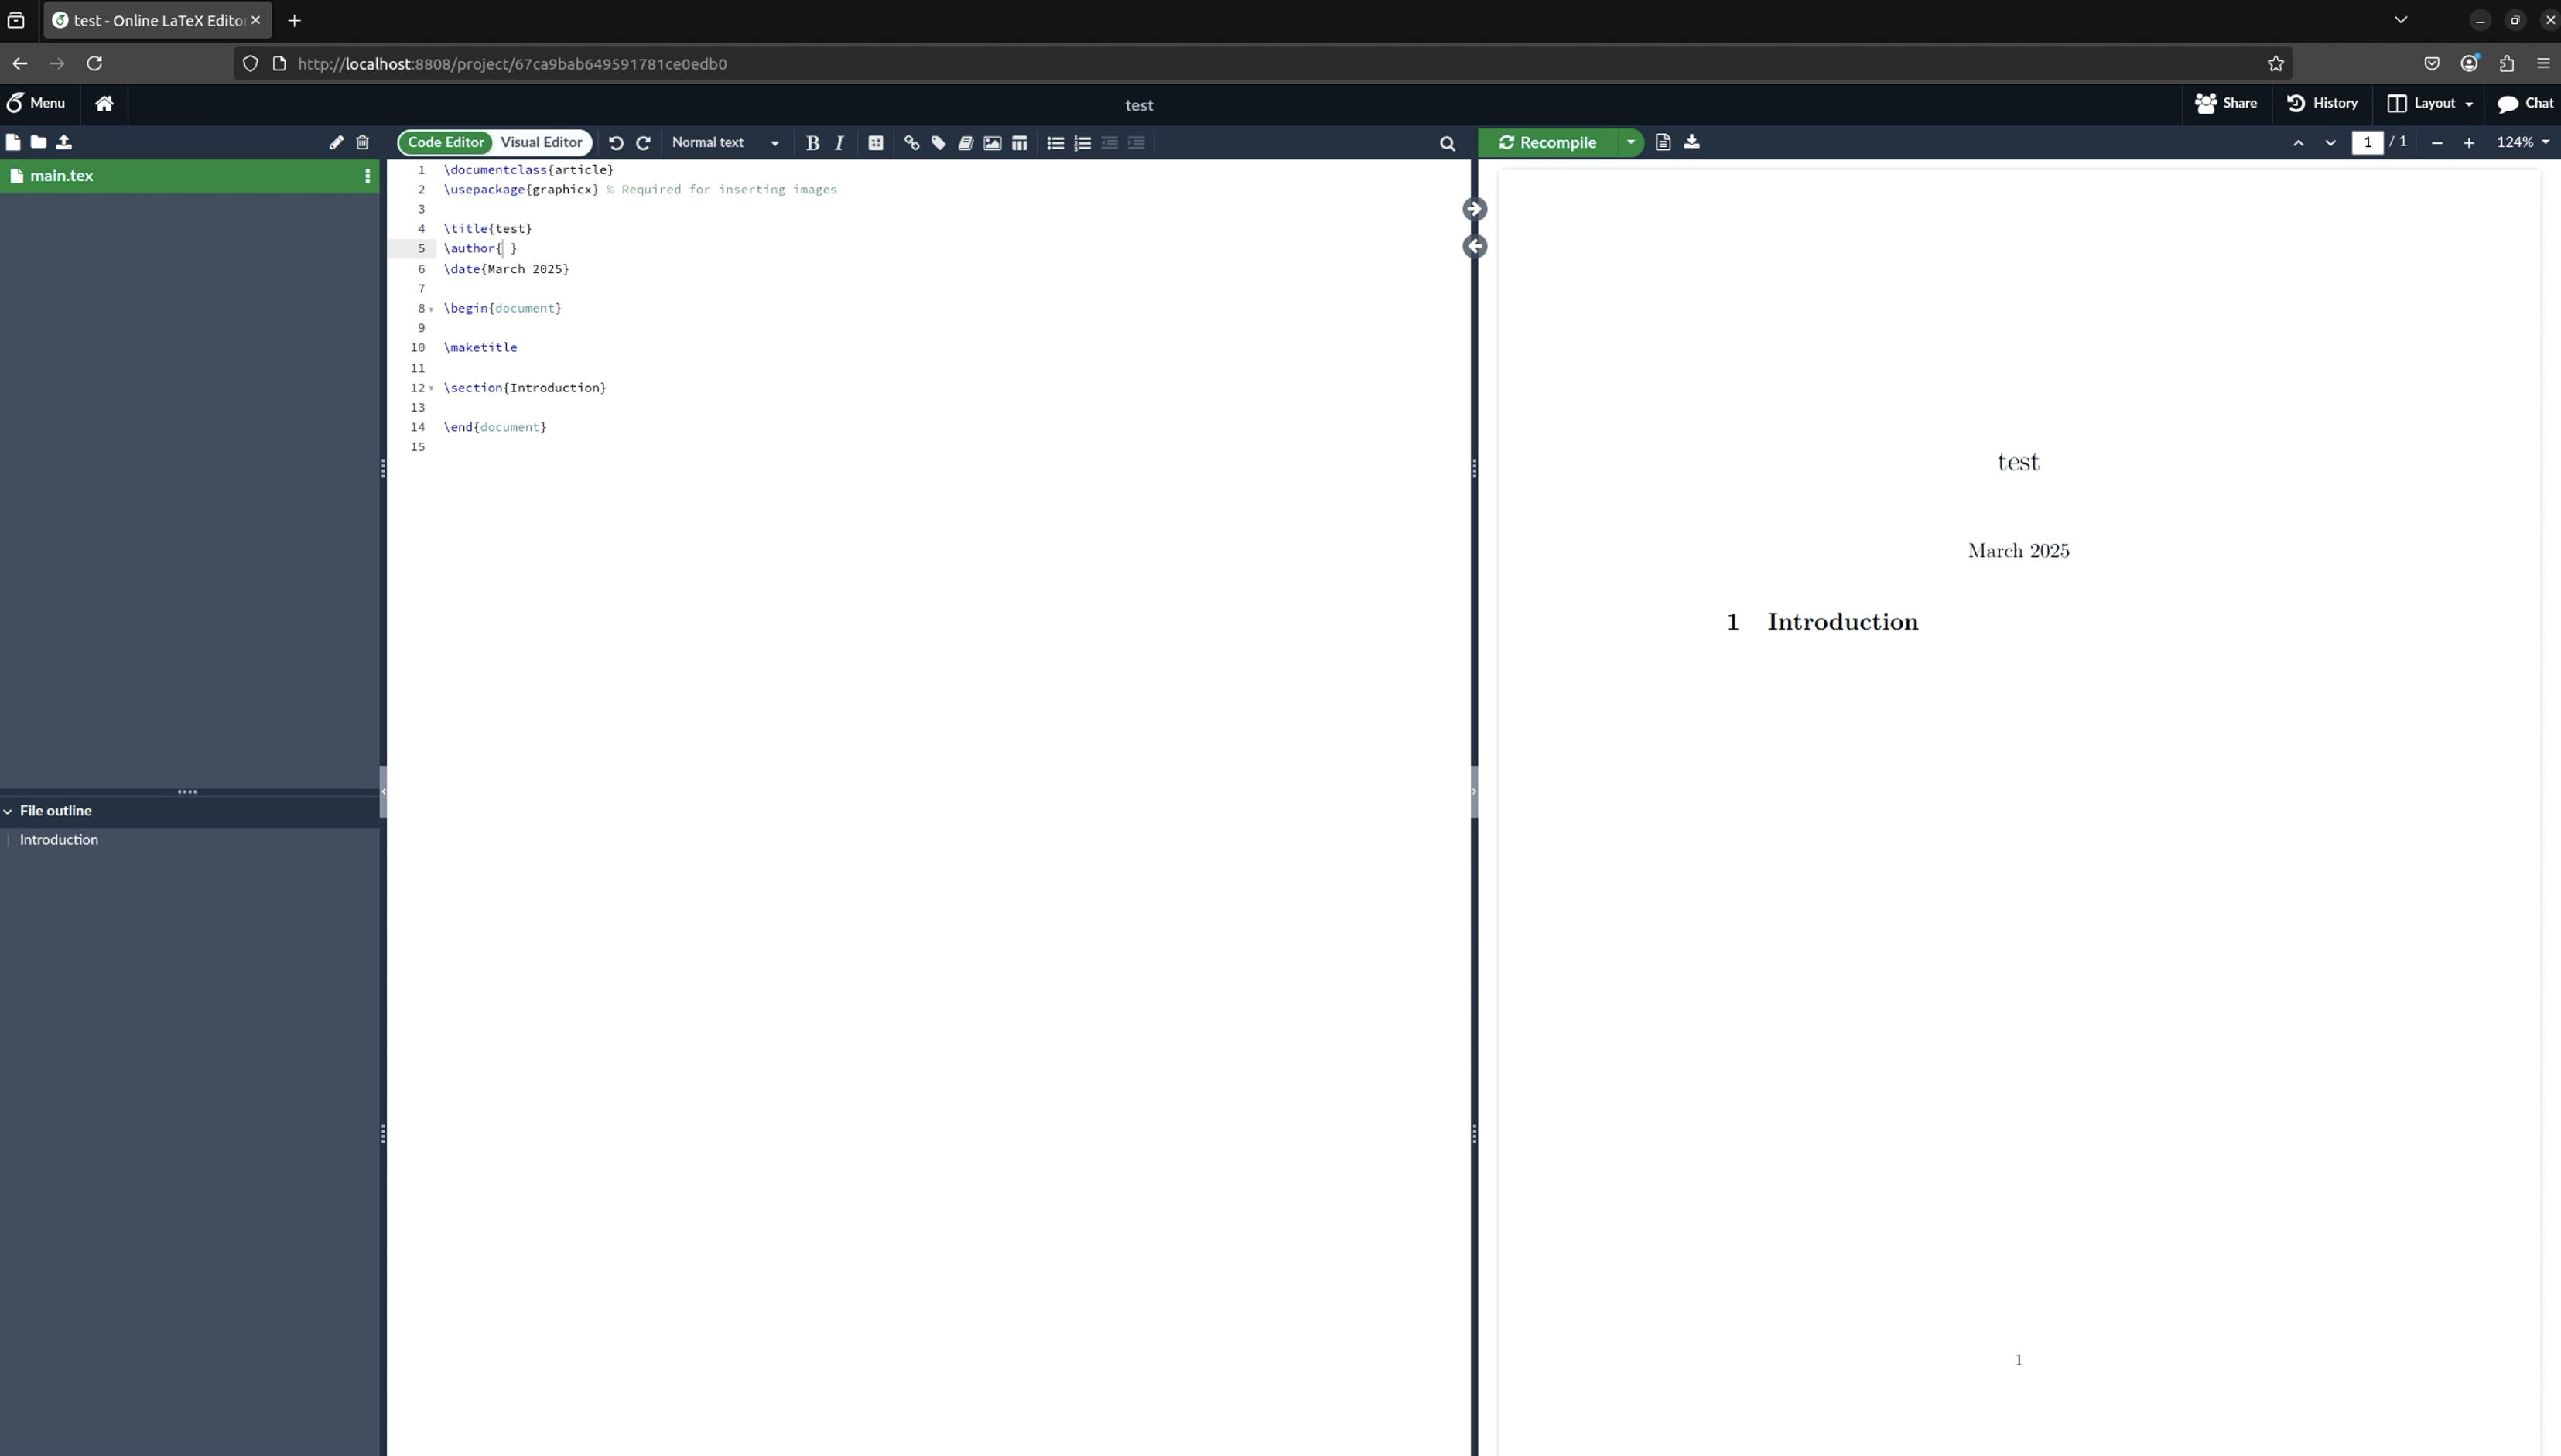
\includegraphics[width=0.8\linewidth]{images/Pasted image 20250307161002.png}

\subsection{完全なTeXLiveとCJK言語サポートのデプロイ}
デフォルトのShareLaTeXイメージには最小限のTeXLiveのみが含まれています。完全版をインストールするには以下の手順に従ってください:

\begin{enumerate}
\item コンテナ内部でコマンドラインに入る
\begin{lstlisting}[language=bash]
docker exec -it sharelatex-test /bin/bash
\end{lstlisting}

\item \texttt{tlmgr}の更新と完全版TeXLiveのインストール
\begin{lstlisting}[language=bash]
tlmgr update --self
tlmgr install scheme-full
\end{lstlisting}
※ 完全なTeXLiveのインストールには長時間を要します。ネットワーク環境とサーバ性能に応じて、コーヒーを飲むか昼食を取ることを推奨します。

\item CJK文字エンコーディングライブラリと言語サポートのインストール
\begin{lstlisting}[language=bash]
apt update
apt install -y latex-cjk-all texlive-lang-chinese texlive-lang-japanese texlive-lang-korean texlive-lang-english fonts-noto-cjk
\end{lstlisting}
\end{enumerate}

\paragraph{Google Notoフォントについて}
Google Notoフォント(Noto CJK)は中国語・日本語・韓国語の文字を統一デザインでサポートするオープンソースフォントです。以下の特徴を持ちます:
\begin{itemize}
\item 日本語:Noto Sans CJK JP/Noto Serif CJK JP
\item 簡体字中国語:Noto Sans SC/Noto Serif SC
\item 繁体字中国語:Noto Sans TC/Noto Serif TC
\item 韓国語:Noto Sans KR/Noto Serif KR
\end{itemize}

\paragraph{XeLaTeXの設定}
LaTeX文書でCJK文字を正しくレンダリングするには:
\begin{itemize}
\item 左上メニューからコンパイルツールを\texttt{XeLaTeX}に変更
\item 文書先頭にパッケージを追加:
\begin{lstlisting}[language=TeX]
\usepackage{xeCJK}
\end{lstlisting}
\end{itemize}

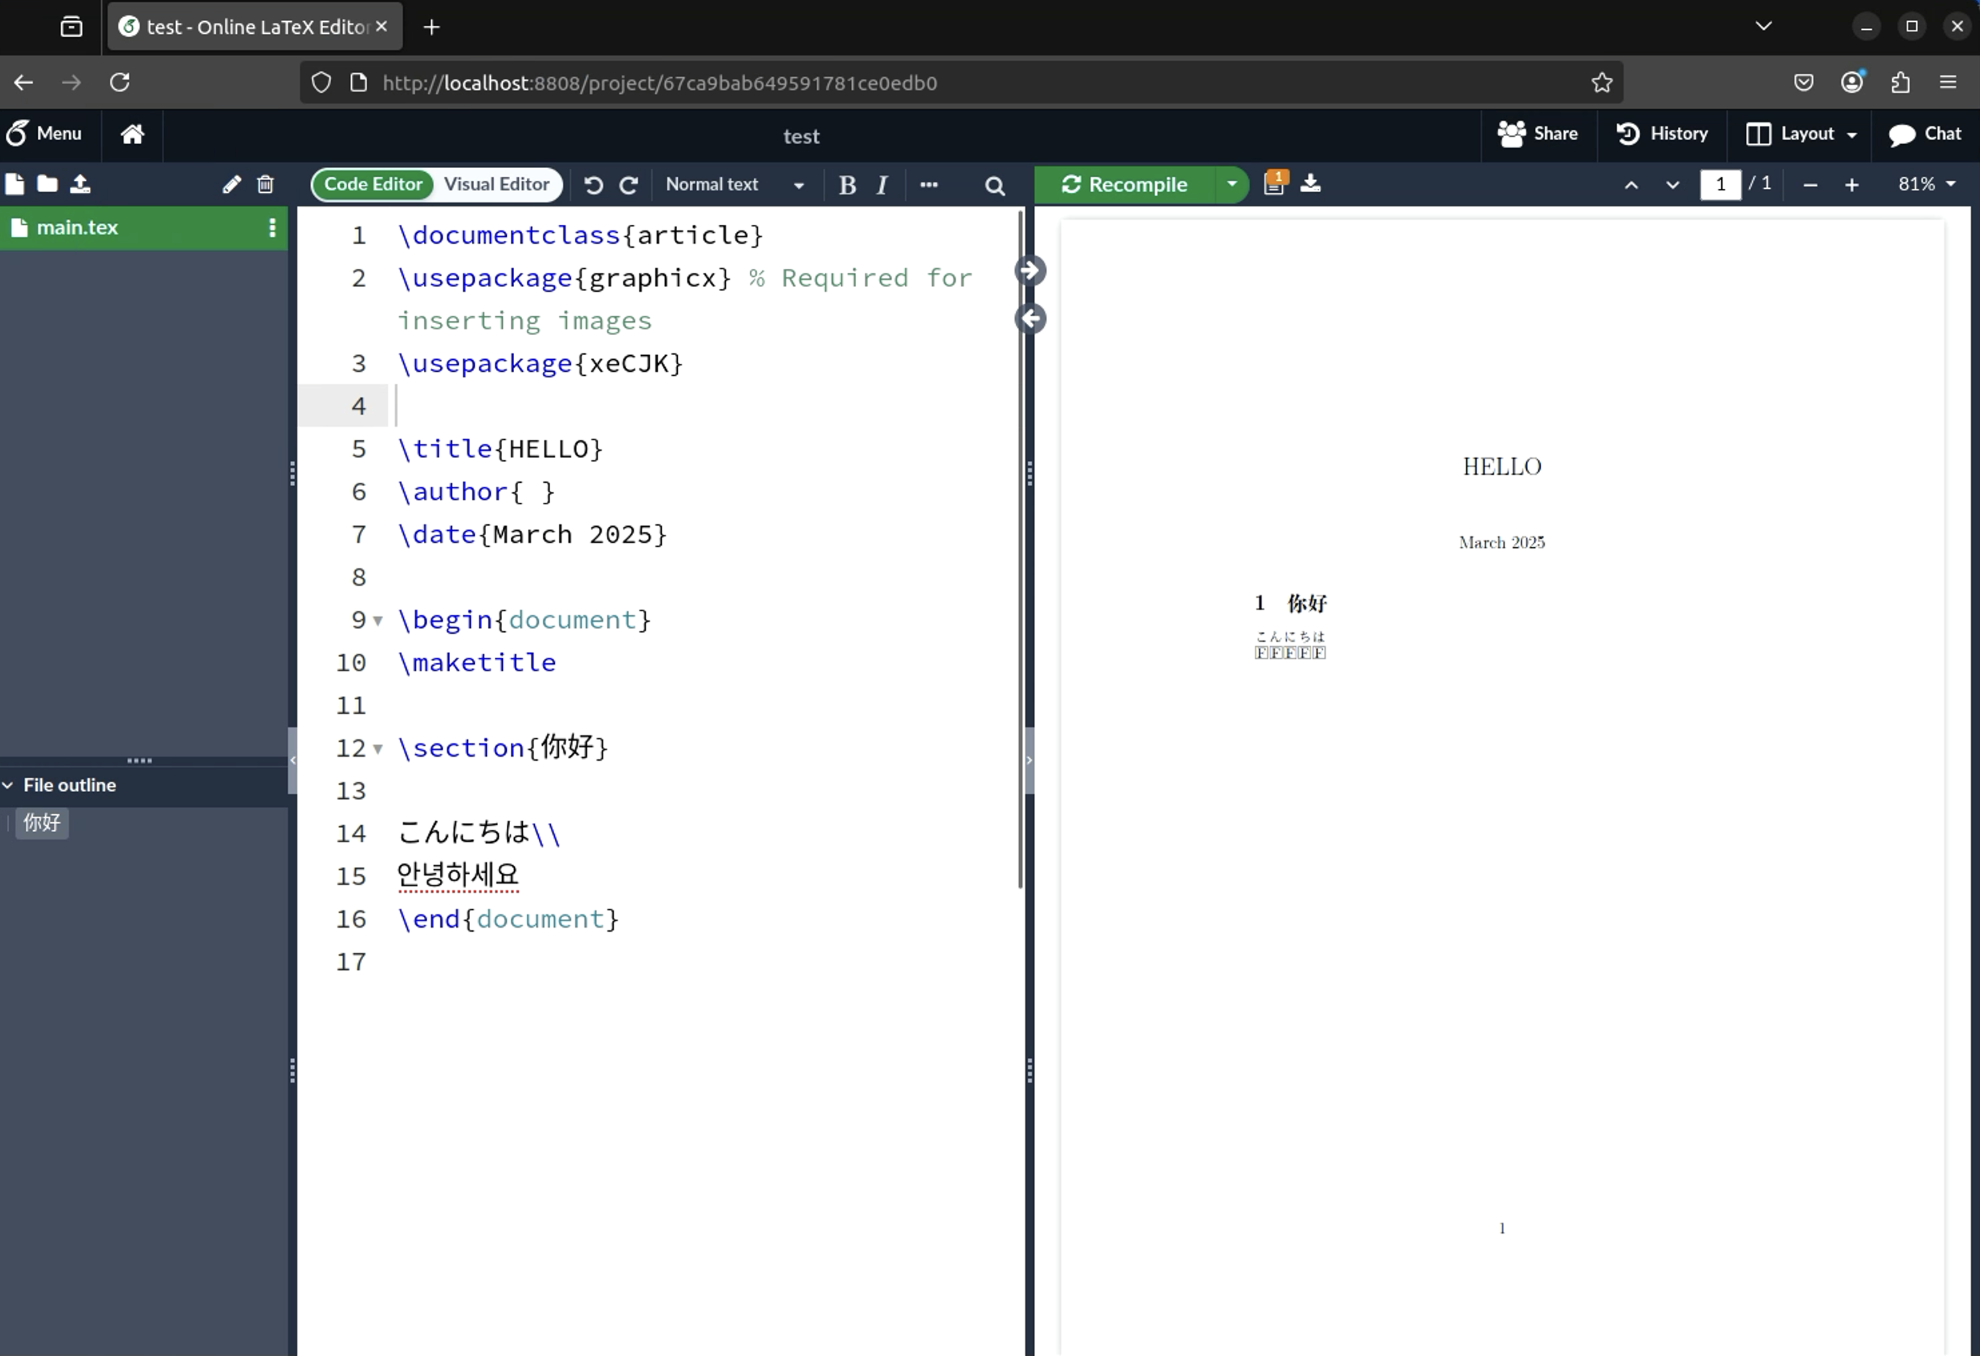
\includegraphics[width=0.8\linewidth]{images/Pasted image 20250307175237.png}

\paragraph{韓国語の追加設定}
韓国語を使用する場合はフォントを明示的に指定する必要があります:
\begin{lstlisting}[language=TeX]
\usepackage{kotex}
\setmainhangulfont{Noto Serif CJK KR}
\end{lstlisting}

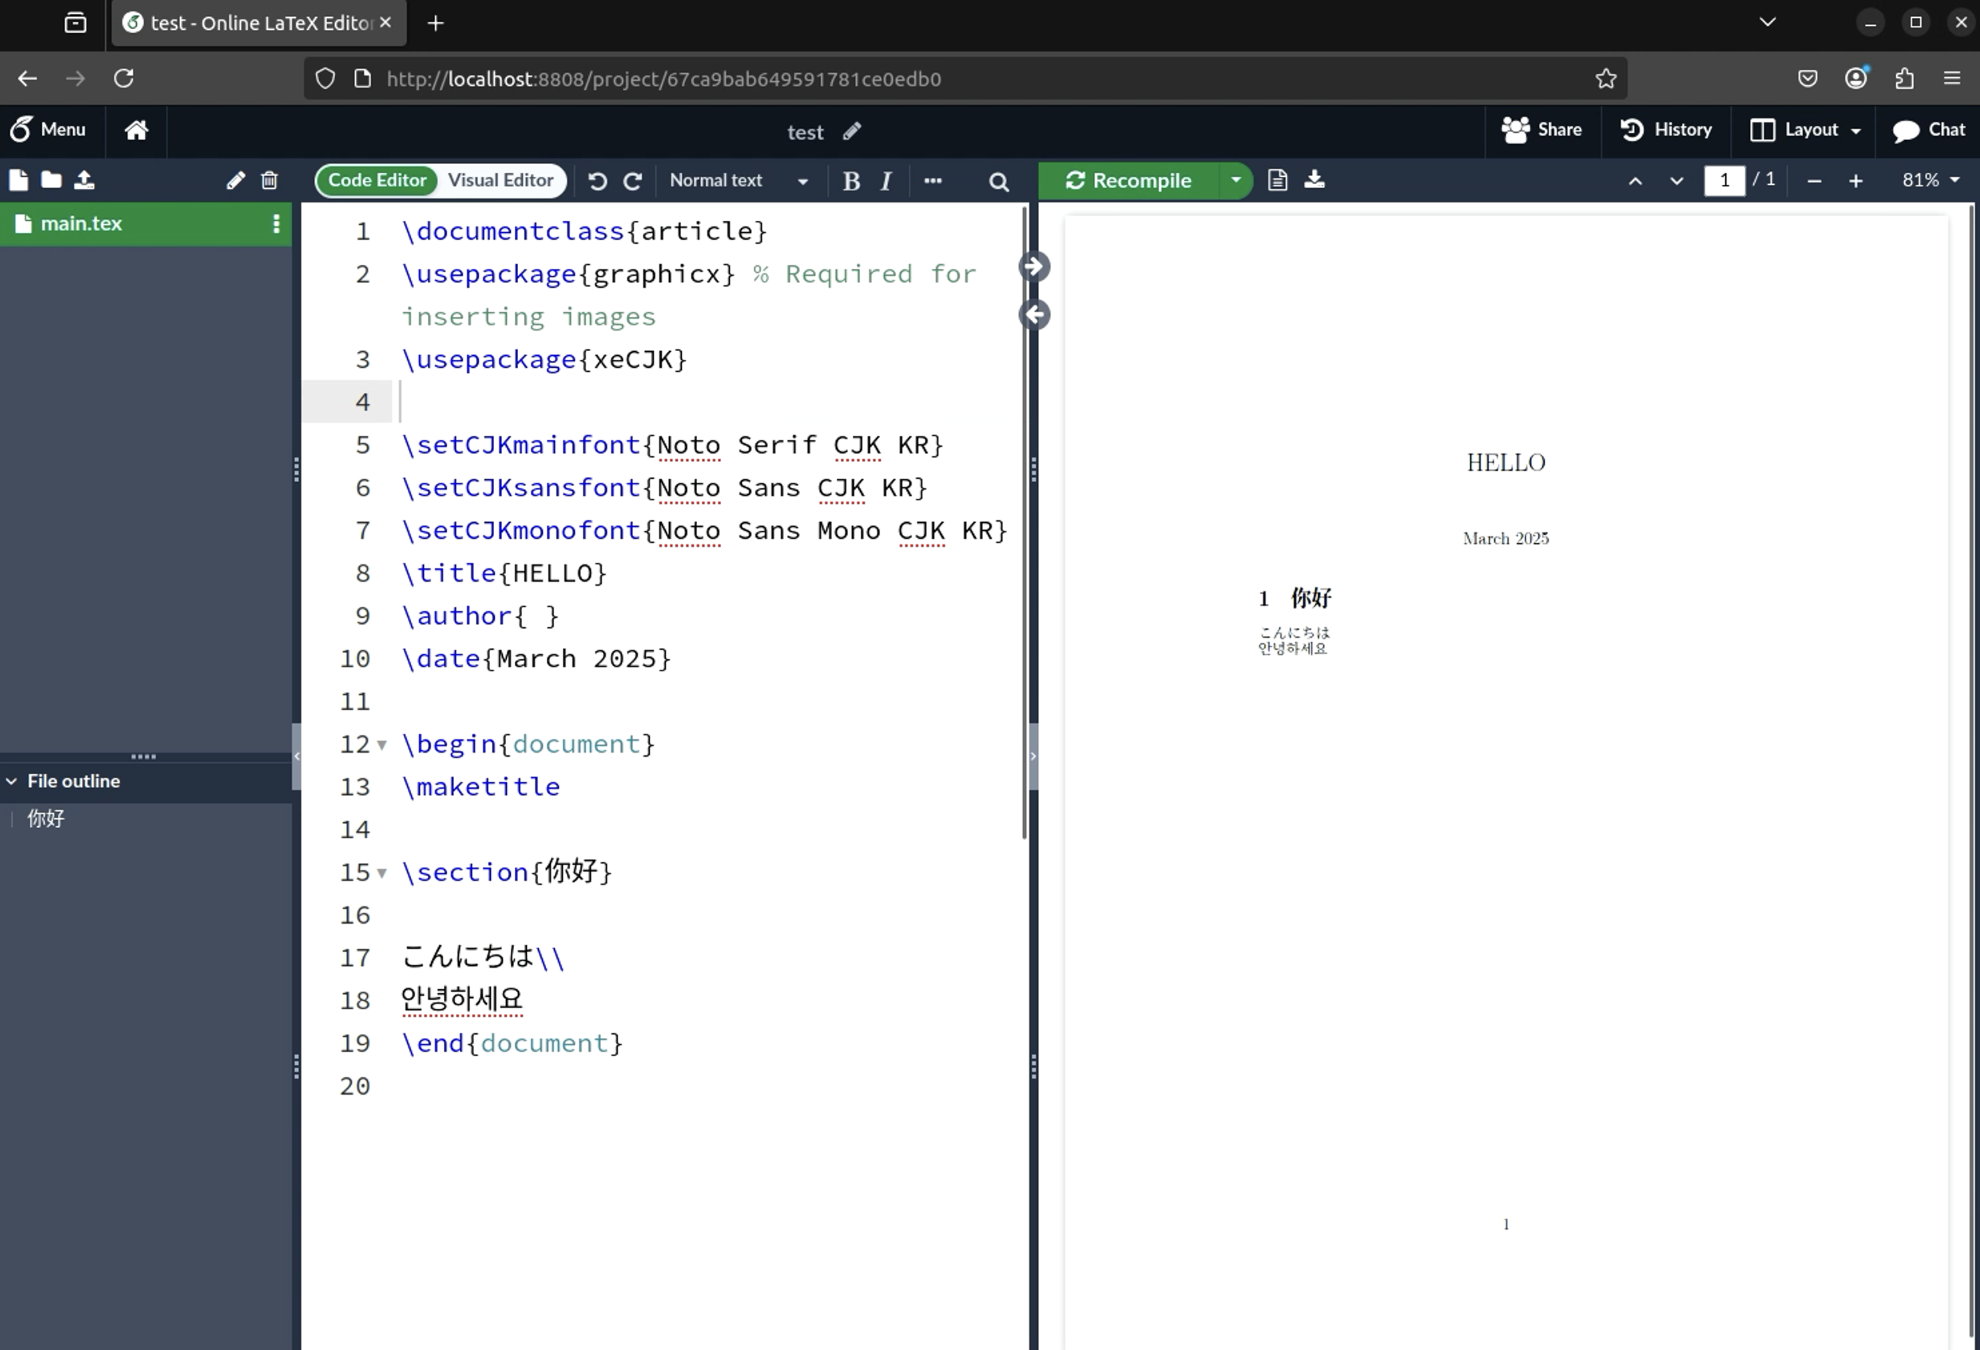
\includegraphics[width=0.8\linewidth]{images/Pasted image 20250307180333.png}

また、日本語や中国語が正しく表示できない場合は、対応するフォントを指定することで正常に表示できるようになります。
    
\paragraph{その他の機能}
ファイル管理やマルチユーザー協業機能など、その他の実用的な機能はOverleaf公式Web版と同様に動作します。


\section{Dockerコンテナを用いた開発環境の構築}
続いて統合開発環境(IDE)のDocker連携機能について説明します。JetBrains社の各種IDEやMicrosoft社のVisual Studioなど、多くのIDEがDocker開発機能を統合または拡張可能ですが、これらは通常追加のDockerリモートサポート購入が必要です。研究チームがクラスタやサーバ上でDockerを運用する場合、必ずしも最適な解決策とは言えません。そこで、Microsoft社が提供するVisual Studio Code(以下VS Code)を推奨します。

\subsection*{Visual Studio Codeについて}
VS Codeはオープンソースの軽量エディターで、以下の特徴を持ちます:
\begin{itemize}
\item クロスプラットフォーム(Windows/macOS/Linux)対応
\item 豊富な拡張機能エコシステム
\item 組み込みターミナルとGit統合
\item 無料で商用利用可能
\end{itemize}

VS Codeのインストール手順は容易なため本稿では割愛します。次に、VS CodeにDocker拡張機能をインストールしてください。公式ガイド「\href{https://code.visualstudio.com/docs/containers/overview}{Docker in Visual Studio Code}」を参照してください。

\subsection{PyTorchコンテナの実行例}
\begin{lstlisting}[language=bash]
docker run --name pytorch-test --mount type=bind,src=/home/username,dst=/root/ --gpus all --ipc=host -it nvcr.io/nvidia/pytorch:xx.xx-py3
\end{lstlisting}

\paragraph{コマンドパラメータ解説}
\begin{itemize}
\item \texttt{--mount type=bind,src=/home/username,dst=/root/} :
ディレクトリマウント。ホストOSの\texttt{/home/username}ディレクトリをコンテナ内の\texttt{/root/}にバインドマウント(双方向同期)。

\item \texttt{--ipc=host} :
IPC名前空間共有。コンテナがホストOSのプロセス間通信(Inter-Process Communication)リソースにアクセス可能にします(共有メモリを使用するアプリケーションに必須)。

\item \texttt{--gpus all} :
GPUデバイス割当。NVIDIA GPUをコンテナに全デバイス公開(NVIDIA Container Toolkitの事前インストールが必要)。

\item \texttt{nvcr.io/nvidia/pytorch:xx.xx-py3} :
コンテナイメージ指定。\href{https://docs.nvidia.com/deeplearning/frameworks/support-matrix/index.html}{NVIDIA NGCカタログ}で提供されるPyTorch公式イメージ(\texttt{xx.xx}はCUDA/PyTorchバージョン組み合わせ)。
\end{itemize}


\paragraph{\texttt{--mount}と\texttt{--volume}の違い}
前章で使用した\texttt{-v}(\texttt{--volume}の省略形)との主な差異:
\begin{itemize}
\item \texttt{--volume}: Docker管理のボリュームを使用(データ暗号化可能・外部アクセス困難)→ アプリ配布/機密データ向け
\item \texttt{--mount}: ホストOSのファイルシステムを直接マウント(双方向リアルタイム同期)→ 開発環境向け
\end{itemize}

\subsection{VS Codeとの連携手順}
コンテナ起動後、VS CodeのDocker拡張機能から該当コンテナを右クリックし「Attach Visual Studio Code」を選択します。新規ウィンドウが開いたら、作成済みのコンテナを選択してください。

\begin{enumerate}
\item プロジェクトディレクトリ(Sec.5.1で取得したディレクトリ)を開き、\texttt{./notebook/mnist.ipynb}ファイルを選択
\item カーネル選択で「Python Environments」→「Global Env」を指定
\item 自動表示されるポップアップから「Python + Jupyter拡張機能」をインストール
\item インストール完了後、再びファイルを開いてカーネルを選択
\end{enumerate}

\paragraph{\texttt{torch}インポートエラー/GPU認識不良時}
コンテナ内で\texttt{nvidia-smi}を実行した際、以下のエラーが発生する場合:
\begin{lstlisting}
% nvidia-smi
Failed to initialize NVML: Unknown Error
\end{lstlisting}

解決策:
\begin{itemize}
\item コンテナを再起動(前章のGPUデバイスマウント手順を再確認)
\item NVIDIAドライバのバージョンとコンテナの互換性を確認
\end{itemize}

これでJupyter Notebookの編集が可能になります。以降の操作はVS Code上で実施してください。


\end{document}
